\chapter[導入]
{導入}


\chaptermark{Introduction}

%\chapterauthor{Hein Mannaerts}



\begin{abstract}
Lesson abstract goes here
\end{abstract}

Lesson contents go here

\section{通信の歴史}

\subsection{紹介}

量子通信の基礎へようこそ。量子技術高等教育拠点の一つ目のモジュールなんですけれども、量子通信・量子インターネットの最初の段階です。
これは連続で何年間のカリキュラムにあって、これを勉強したら量子通信の専門家になる可能性があります。宜しくお願いします。
今日のレッスンとしては、まずは通信の歴史なんですけれども、これは第1本です。

このモジュールにはいくつかの段階があるんですが、まずは量子力学を
レビューします。それが前提ではないんですが、必要な知識だけは伝えておきます。
そして、エンタングル(量子もつれ)状態のことについて勉強します。
その後は、量子通信の基礎のことを勉強をして、最終的には、量子中継機については、いくつかのレッスンがあって、今回の全てのモジュールです。

コミュニケーションの場合には、もちろん人間の社会は連続で何万年間話をしたり、コミュニケーションしたりしているんですけれども、それが社会が発展するためには必要な技術です。昔は、皆さんは火の周りに集まって、議論したり、話ししたり、音楽やったりとかをしてたんですが、それが個人個人には対面でやってた話とかはありました。現在の状態としては全世界の人々はいろんな人々と繋がって、それが会話できるようになりました。情報を伝えるようになりました。

\begin{figure}[H]
    \centering
    \includegraphics[width=0.9\textwidth]{lesson1/communication.eps}
    \label{図: 1}
    \caption{通信の進化}
\end{figure}

どうやって、\emph{Local Communication} から \emph{Global Communication} までには技術が進化されているでしょうか。それが今日のテーマです。
もちろん、一番簡単な手法としては直接情報を伝える事です。
\subsection{直接通信}
例えば、数千年前にはギリシアで有名なことなんですけれども、マラソン(Marathon)の戦場で、メッセージを伝えました。現説としては、マラトンという町からアテネ(Athens)までの距離で、誰か走ってメッセージを持っていったんです。実はアテネからスパルタ(Sparta)までの225kmの距離を1日で走って行ったんです。当時では素晴らしいスピードと思われていました。

しかし、通信が数百キロに1日かかることは現代だとしたら遅いです。

もう一つの例としては、鳩の足にメッセージを薄い軽い紙に書いて、それを鳩の足につけて、その鳩は、現地から自宅まで帰させます。

自分が旅をする場合には、ハト何羽か持っててケージに入れて、現地から自宅にメッセージを送りたい場合には、送ることができます。
鳩は1600km離れた自宅まで飛べ等れます。速度は平均時速95キロぐらいで最も優秀な鳩は時速160キロまでいけます。

最後に、米国の有名な通信の手法について述べたいと思います。「ポニーエクスプレス」は1年間ぐらいしか営業してなかったんですが、手紙を運びながら10日で4000km(東海岸から西海岸まで)まで走れました。メッセージを軽い紙に書き、封筒に入れ、ポニーエクスプレス社に渡し、ライダーがそれを持って馬に乗り、
馬が疲れるまで走る通信方法でした。
% insert photo here
\begin{figure}[H]
    \centering
    
\includegraphics[width=0.6\textwidth]{lesson1/ponyexpress.eps}
    \label{図: 1}
    %\justification=<centering>
    \caption{ポニーエクスプレスの紋章}
\end{figure}

中継場のところでは止まって、新しい馬に乗り換えたりして、そのまま疲れるまで走ります。そうすると、10日間ぐらいには、その4000km でもメッセージを伝えることができました。
しかし、言った通りこの制度はおよそ1年間しかやってなかったんです。この次の技術の方が進化してたので、メッセージを伝えることがより早くできるようになりました。この「次の技術」は、電気を使ったメッセージの通信の手法をです。

直接メッセージを伝えることはやはり二つの非常な弱点があります。
\begin{enumerate}
    \item 「遅い」:現代は地球のある所から地球の反対側まで数百ミリかからのが常識と思われてます。鳩や馬は敵えません。
    \item 「信頼性」:メッセージを落としたり、メッセンジャーが暗殺されたり病気になったり、やむをえず色々な危険があります。
\end{enumerate}

\subsection{光学通信}

次のステップは、光を使ってメッセージを伝えることです。メッセージシステムを使う前には、その信号の意味などを決めなきゃいけないんですが、それがSender (送信者)とRecipient (受信者)の間にはメッセージの意味を伝えることにはしなければならない。
例えば、中国の万里の長城。この数千キロの鉄壁は北側からの攻撃から守るためにいろんなメッセージを伝える必要があったのです。どうやってメッセージを送るといえば、壁上の各塔から攻撃してくる人が見えたら、その塔の上に火をつけてました。
% insert photo here
\begin{figure}[H]
    \centering
    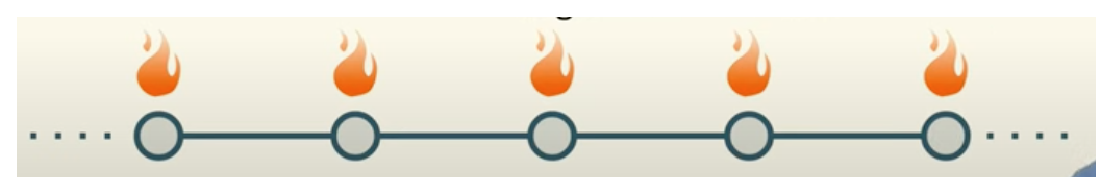
\includegraphics[width=0.9\textwidth]{lesson1/万里の長城.eps}
    \label{fig: 1}
    \caption{万里の長城}
\end{figure}

その火をつけて、隣の塔で火を付けることが見えたら、自分の塔に火をつけて、連続するとメッセージを広く送れます。その火の意味は「攻撃されてます」「手伝っていただけますか」の状態です。物理的には人がポイントAからポイントBまで行く必要がなく、火を見るだけで通信が可能だったので、結構長い距離の通信ができるようになりました。

しかし火をやっているかやってないか、それでそれがメッセージになっているだけです。基本的に伝えると、イエスとノーしかないです。

もうちょっと、洗練されたやり方としては、ナポレオンの時代、19世紀なんですがフランスでは、ナポレオンの「セマフォ」。
% Insert photo here
\begin{figure}[H]
    \centering
    \includegraphics[width=0.9\textwidth]{lesson1/napoleon.eps}
    \label{fig: 1}
    \caption{ナポレオンのセマフォ}
\end{figure}

日本語では「腕木通信機」と言いますけれども、見える通りにこれが小さい家の上に、木材で作られている装置を作ってやるんですが、これが棒があって、腕があって
腕の位置については、これが「A」でこれが「B」とか、いろんなやり方があったんです。一つのメッセージだけを伝えるんじゃなくて、汎用的なメッセージを伝えるのに使えるんですよね。これがフランス全国だけじゃなくて、ヨーロッパ大陸の中で使ってたんです。しかし、腕木を動かして、メッセージ送るためには、紐も引っ張ったりしていたので、家の中に人が必要です。そうすると、中継所と中継所の間には10キロぐらいメッセージを通信できるようにして、連続でそれが複数のところに繰り返して繰り返して、繰り返すことにしました。良いポイントはいくつかあるんです。
\begin{enumerate}
    \item 「早い」:先に出た中国の万里の長城の火と比較すると、スピードはかなり早いでしょう。パリからベネチアまでには数時間やパリからフランスの東側にあるストラスブールまで1時間で通信できるようにはなりました。
    \item 「信頼性」:メッセージを落としたり、メッセンジャーが暗殺されたり病気になったり、やむをえず色々な危険があります。
\end{enumerate}
まずは
しかし、弱点もありました。
\begin{enumerate}
    \item 「天候」:天気が悪い日には使えないし夜にも使えないものなんです。
    \item 「人手」:紐とレバーとかひっぱたりとかしなければならないから、結構力は必要です。さらに、人間はよく間違えたり、壊したります。
\end{enumerate}
弱点もありました。
これが天気が悪い日には使えないし

\subsection{電気通信}
さて、次のステップは
こういう視覚的システムじゃなくて、電子信号を使うことになりました。
一番有名な手法としてはとしては、モールス信号ですね。
% insert photo here. TODO: How to make these side-by-side?
\begin{figure}[H]
    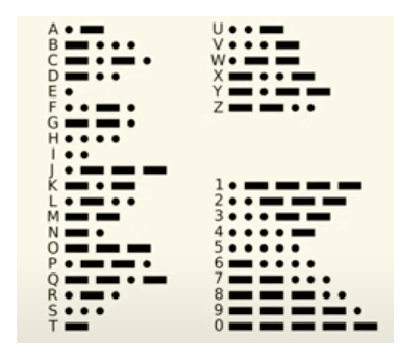
\includegraphics[width=0.3\textwidth]{lesson1/morse.eps}
    \label{fig: 1}
    \caption{モールス信号}
\end{figure}
\begin{figure}[H]
    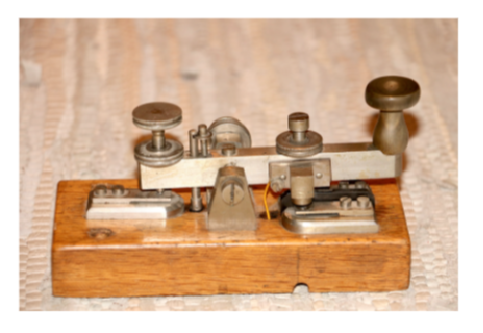
\includegraphics[width=0.3\textwidth]{lesson1/morsekey.eps}
    \label{fig: 1}
    \caption{モールスキー}
\end{figure}
\iffalse
\begin{figure}
    \centering
    \begin{minipage}{0.45\textwidth}
        \centering
        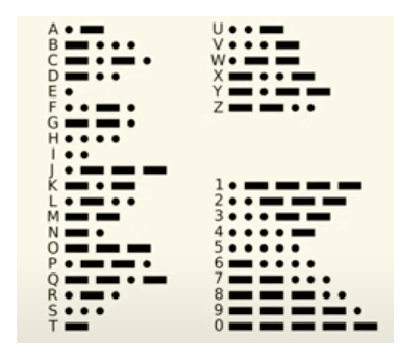
\includegraphics[width=0.9\textwidth]{lesson1/morse.eps} % first figure itself
        \caption{first figure}
    \end{minipage}\hfill
    \begin{minipage}{0.45\textwidth}
        \centering
        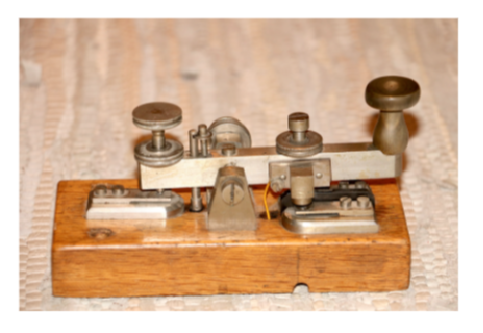
\includegraphics[width=0.9\textwidth]{lesson1/morsekey.eps} % second figure itself
        \caption{second figure}
    \end{minipage}
\end{figure}
\fi


モールス信号が電子信号を使うことにして、
こういう機械を使ってたんですね。パタパタと打ち込むと、それが
電子の回路が繋がったり離れたり外したりするとこれが信号のオンとオフをになることなんですが、そうすると短点と長点(短いものと長いもの)で2つの信号の種類があるんですが、英語では、「ダッシュ、ドット、ダッシュ、ドット」と読み方をするんですが、日本語では「ツー、ドン」だと思います。
「ツー、ドン、ツー、ツー、ドンドン」
すると、メッセージが伝えるようになります。そういうふうに読み、アルファベット順にできます。長いメッセージと短いメッセージがあって、一番良く使われているものは
アルファベットのレターとして「E」なので、それ一番短いメッセージです。あまり使われてないアルファベットの記号はそれ長いメッセージになっているんですが、それが「X」 とか「G」 とか、そういうふうなんです。この技術を利用し、数分でアメリカの東海岸から西海岸までメッセージを通信できるようになりました。さっきのシステムと同様に、中継所を使わなければならなかったんですが、一つの信号は数千キロぐらいまで通信できるようになってなかったので、途中で誰かが聞いて、書き出し、同じメッセージをもう1回次の中継所まで送る制度になってました。この新技術はさっき話したポニーエクスプレスやナポレオンの腕木通信機が使われなくなった原因です。もちろん、モールス信号にも短所があります:
\begin{enumerate}
    \item 「難易度高い」:違う通信手法と比べると、訓練も必要なんです。訓練されていない人ははあまりメッセージがを読んだりとか聞いたりとかできないものなんですよね。
\end{enumerate}

そうすると、続きの技術としてには 電話になっていたんですが、その電話が
\textbf{初めて長い距離でボイス}の通信ができるようになりました。自分の声で通信でできるようになりました。これは一番最初の方は、ポイントツーポイントなんですが、 Aさんの家からBさんの家にメッセージを伝えるようにしたいなら、その間には直接電線を引っ張らなきゃいけなかったです。もちろんこの方法には限界があるんです。
% Insert point-to-point pic here
\begin{figure}[H]
    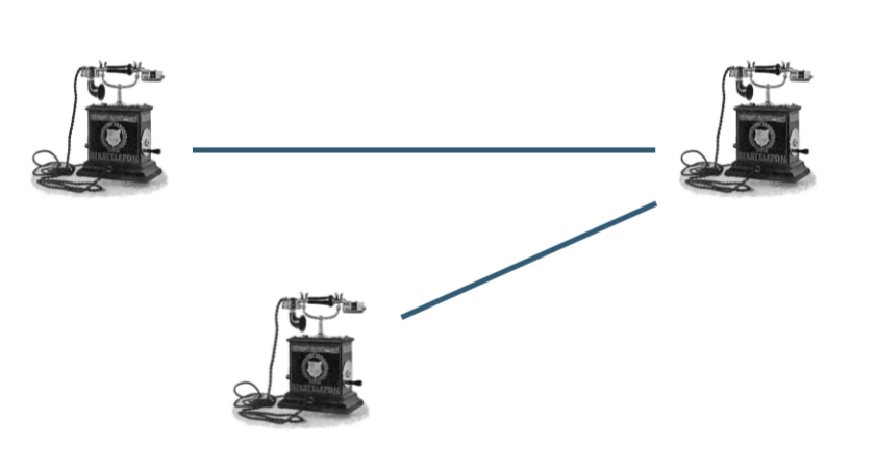
\includegraphics[width=0.8\textwidth]{lesson1/pointpoint.eps}
    \label{fig: 1}
    \caption{ポイントツーポイント手法}
\end{figure}


その後の進化としては、ネットワークの真ん中にはスイッチボードという概念のを作って、それを入れたんですが、そうすると自分の家かからそのスイッチボードのところに繋がって、最初にはスイッチボードのところに誰かが電話が出て、「じゃあ、Aさんお願いします」と言って、そのスイッチボードのオペレータが自分の家とAさんの家と繋げることで直接つながることになったんです。
% Insert switchboard pic here.
\begin{figure}[H]
    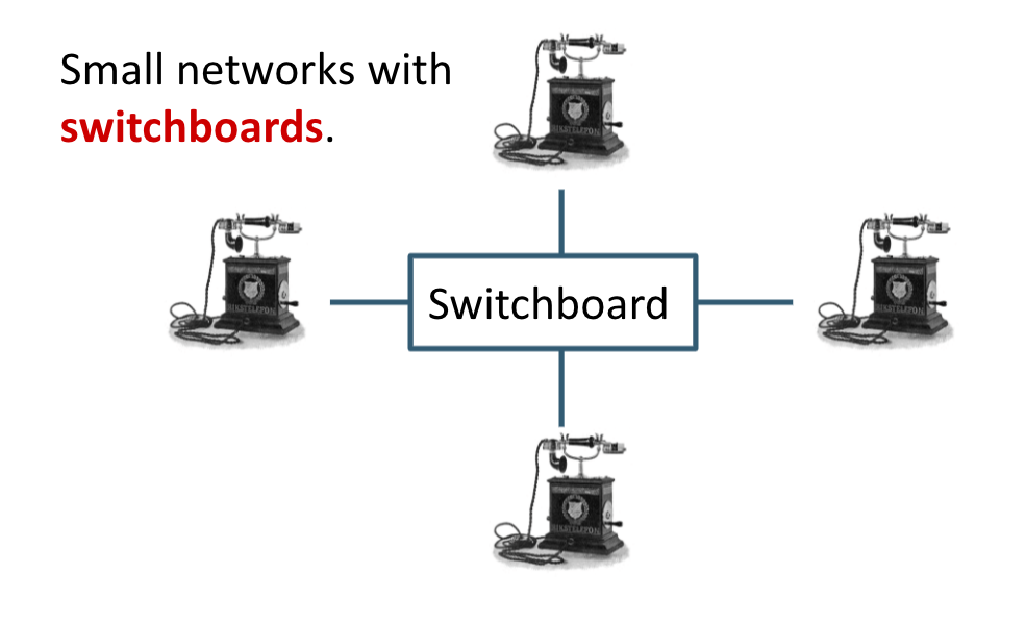
\includegraphics[width=0.8\textwidth]{lesson1/switchboard.eps}
    \label{fig: 1}
    \caption{スイッチボード手法}
\end{figure}
そうするとだんだん広がって、あっという間に世界的規模ぐらいになったんですよね。
その後は、人間のスイッチボードオペレーターが機械に変更しました。
\subsection{インターネット}
次のステップが今の使っているインターネット。インターネットというものが、全世界規模と地球規模の「ネットワーク of ネットワークス」なんですよね。
% insert internet pic here
\begin{figure}[H]
    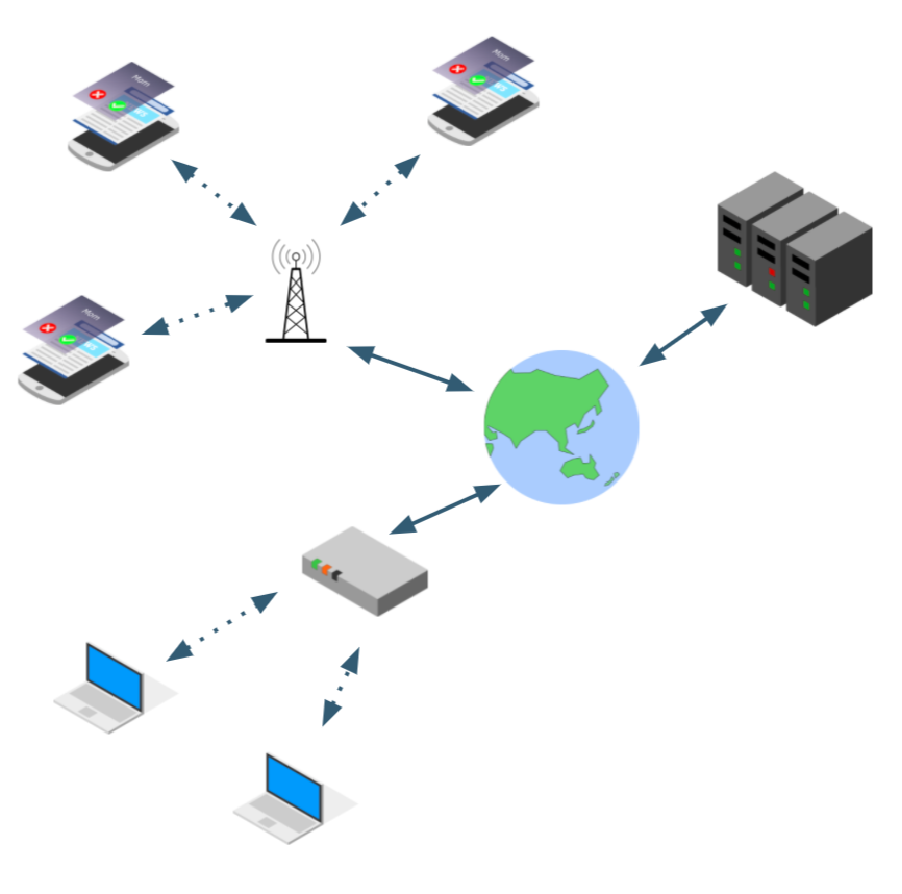
\includegraphics[width=0.8\textwidth]{lesson1/internet.eps}
    \label{fig: 1}
    \caption{インターネット}
\end{figure}
各ところにはネットワークがあって、そのネットワークとネットワークの間の通信があって、それがインターネットワークと呼んで、それを短く呼ぶと「インターネット」になって全世界の一つの通信できるようになりました。
これが例えば、携帯電話のタワーから、自分の持っている携帯からタワーまで通信して、その後はインターネットルーターという機械まで繋がって、その後は向こう側にあるサーバーコンピューターに繋がって、Googleに繋がったりとか、Amazonにつながったりとか
いろんなサービスに繋がることができます。
音声ビデオ、エンターテインメントのいくつかの種類なんですけど、もちろんそれがインフォメーションサービス、これが銀行とか電子メールとか、人と人と、サービスまでの繋がりとかそれが「P2P」、「BtoB」いくつかの略語があって、それがいろんなコミュニケーションのパターンになっているでしょう。このインターネットが良いのは、世界の一番重要な通信基盤になっているんですよね。いくつかのアプリケーションができるようになりました。
% insert picture here
\begin{figure}[H]
    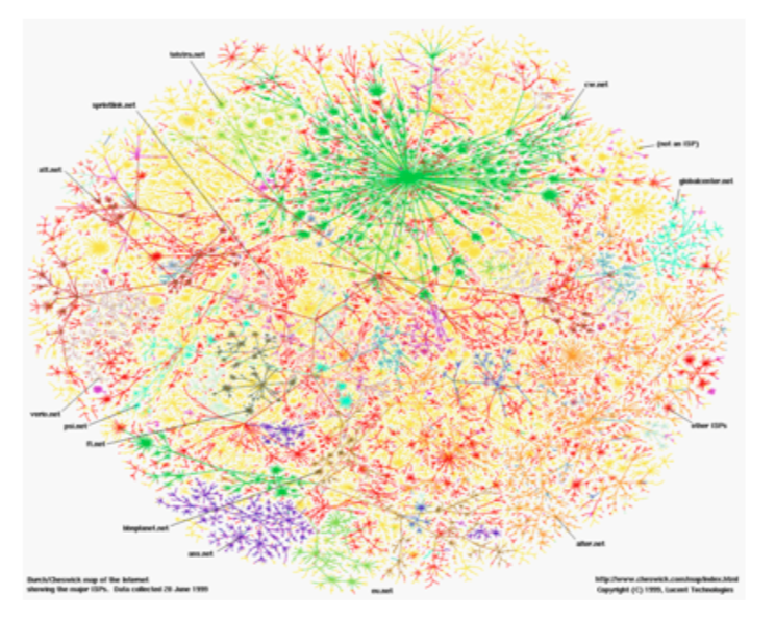
\includegraphics[width=0.8\textwidth]{lesson1/internetmap.eps}
    \label{fig: 1}
    \caption{ネットワーク of ネットワークス}
\end{figure}
先の言ってた通りでインターネットというのは、「ネットワーク of ネットワークス」なんですが、\textbf{Figure 1.10}が1999年の地図なんですが、この地図では線と点のところ、丸のところがあるんですけれど、それが線が物理的な回路じゃなくて、丸がコンピュータとかノードじゃなくて、丸がネットワーク。線がネットワークとネットワークの間の通信する契約がある状態なんですけども、そうするとこの地図が8万個ぐらいのネットワークに繋がっていると思います。これが、今からこれがこのモジュールのやる、量子通信の基礎のことが、この視点から始まります。

\section{アナログからデジタルへ}

\subsection{紹介}
通信したい場合にはどういうふうに抽象化できるのでしょう。
\begin{figure}[H]
    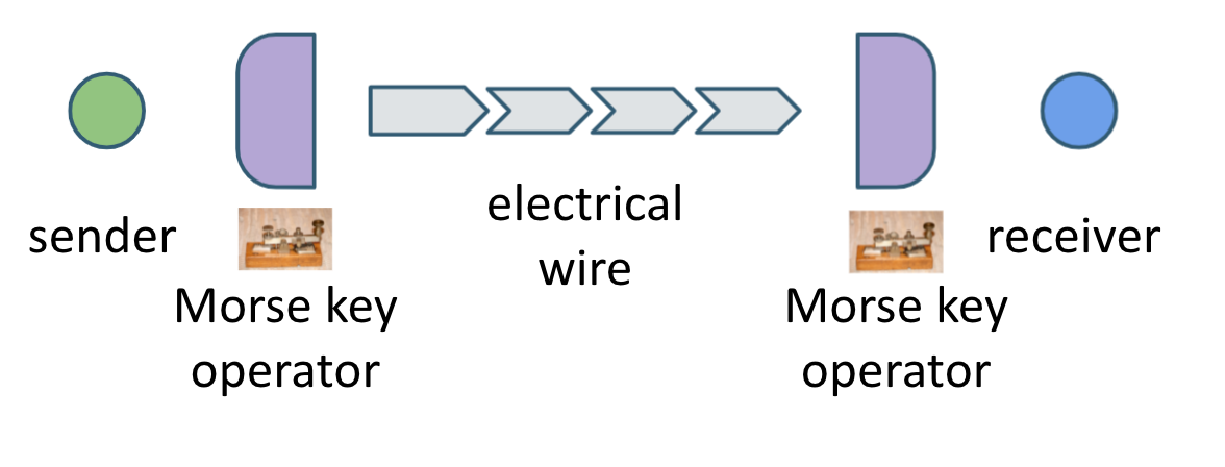
\includegraphics[width=0.8\textwidth]{lesson1/sender_receiver.eps}
    \label{fig: 1}
    \caption{受信者・送信者}
\end{figure}
センダー(送信者)とレシーバー(受信者)といるんですが、そのメッセージを何かでエンコードしなければならない。そうすると、メッセージを伝えて、向こう側にいる相手のいるところにはデコーダーをつけて、メッセージを受信者が読めるようになります。例えば、さっき話をしていたテレグラフ(電信機)としてはモールス信号を使って、それが電子の信号になって、電子の信号が向こう側に届いて向こうにいるモールスキーオペレーターの人が、その電子信号が聞こえて、その後はそれをアルファベットの記号に戻して、メッセージを受信する受信者がそのメッセージを読めるようになります。

さて、こういうふうに考えると、最善の通信手法は何んでしょう?
\subsection{アナログとは?}

我々はアナログの人間なんですが、世界もアナログなんですよね。
「アナログ」と言えば聞く音楽とか、自分の声とかです。あとはタッチ(触る事)です。温度がわかったりとか、材質がきめ細かいだとか、粗いだとかわかったりすることができるのです。あとは、「目」で見えるところ。色もアナログの信号なんですが、それが強いか弱い光か、どんな周波数があるのか、どんな波長があるのか。すると、色も変わるでしょう。
そういう意味で、私たちの世界にはアナログのデータが多いのです。人間はそのアナログのデータの処理は得意なんですね。


さあ、一番最初に考えられる手法としては、メッセージもアナログの手法で通信した方がいいんじゃないですか、とが自然的に思うでしょう。そうすると、これが連続的な信号なのですが、音楽とかあるんですが、そういうアナログ信号が時間が経つと信号の価値が変わるんです。エンコードすると、いくつかのところを使って受信側では、その信号を頂いて、それをデコードすると、そのメッセージが取り戻せるでしょう。

% insert continuous signal picture.
\begin{figure}[H]
    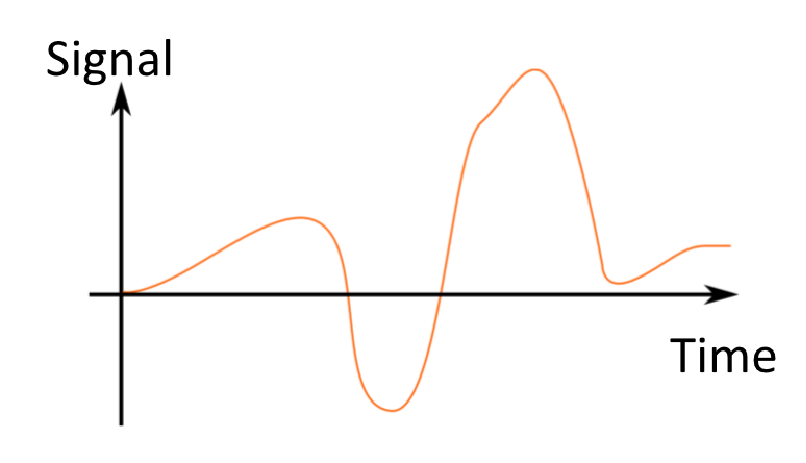
\includegraphics[width=0.8\textwidth]{lesson1/continuoussignal.eps}
    \label{fig: 1}
    \caption{アナログ通信}
\end{figure}

例えば、\textbf{Figure 1.12}のような上がったり下がったりする信号は電話とAMラジオとかでみえる信号の手法です。この場合は、いくつかの問題があるのです:
\begin{enumerate}
    \item 「ノイズ」: ノイズに弱いんです。小さい差があると、それは誤差になる。大きな変化になる場合もありますしそれをコピーすることも難しいんですね
\end{enumerate}

さっきセクション1.1で話してた腕木通信やテレグラフは中継所でメッセージをコピーしてたんですが、それがアルファベットを使ってたから、エラーになる場合は
このアナログの信号より少と思えます。
% insert continuous signal w/ disruptive noise included here. 
\begin{figure}[H]
    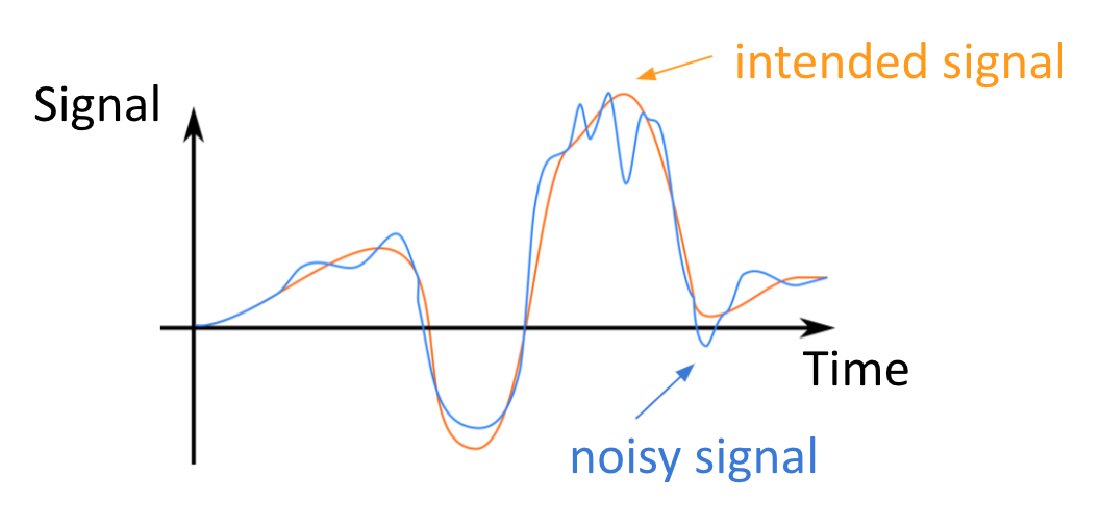
\includegraphics[width=0.8\textwidth]{lesson1/continuous_signal_noise.eps}
    \label{fig: 1}
    \caption{アナログ通信 + ノイズ}
\end{figure}

\textbf{figure 1.13}は\textbf{figure 1.12}のオレンジの信号があったところに、ノイズが入ってきてコピーした場合にこの青い線になる可能性があることを示しています。それは音楽だったら、どのぐらいのノイズが影響するのか。まぁ、機械と信号と人次第なんですが、大きな問題になる場合もありますね。
\subsection{デジタル}
さて、アナログじゃなくてデジタルの信号が使えることは可能なんですが。例としては、腕木通信機とかテレグラフとかを使うと、離散する設定を使うんです。連続信号をデジタルにする場合には、どうすればいいでしょう。
% Insert discrete digital signal pic  w/ t_0, t_1, t_2 here
\begin{figure}[H]
    \centering
    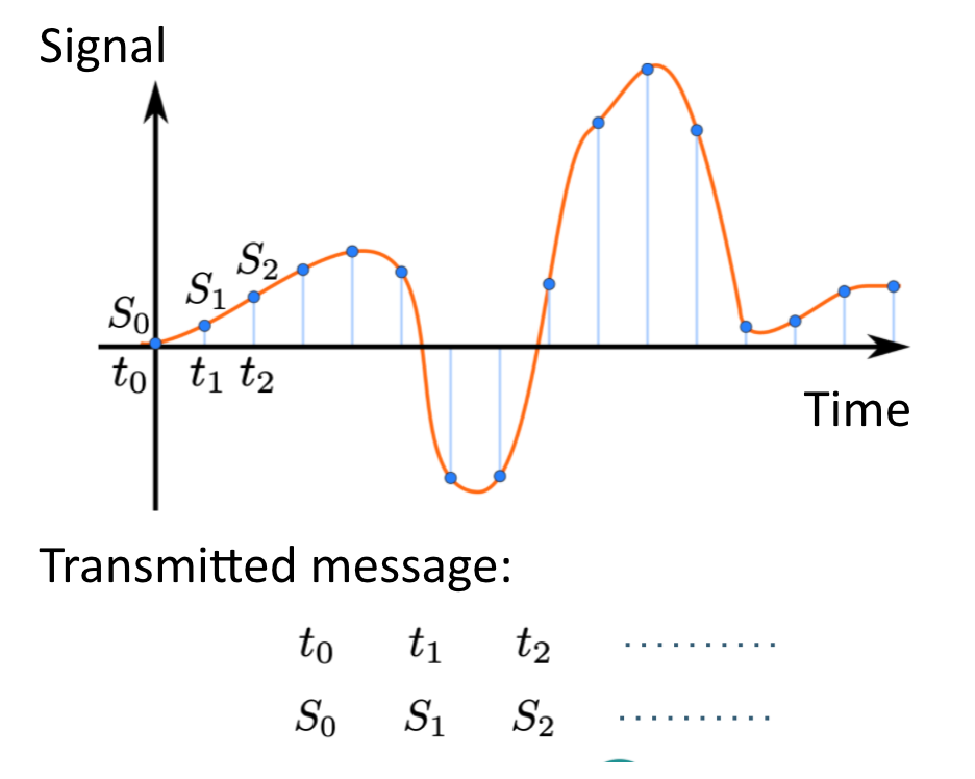
\includegraphics[width=0.8\textwidth]{lesson1/discre_signal.eps}
    \label{fig: 1}
    \begin{center}
        \caption{離散通信}
    \end{center}
\end{figure}
そうすると、\textbf{figure 1.14}で見えるように時間の軸としては信号があるのですが左から右に行くと時間が経つんですよね。すると、その青い所で定時的にその信号を測定しています。その測定されていることが、この青い棒の高さを記録すると信号になるんですね。そうすると、$t_0$、$t_1$、$t_2$には連続でタイムスロットで信号のことに
なるんですが、その場合だったら例えば、$t_0$のところには「$s_0$」になる、$t_1$のところには$s_1$になる、$t_2$のところには$s_2$になるように連続でやります。これの精度が、どのぐらいの頻度でサンプリングすることに依存するんです。低い頻度だと精度が低くなるので、)信号が早く変わってしまう期間には、頻度高くサンプリングすることが必要なんです。
fig[Z]の場合だったら、左側はゆっくり信号が上がってきてるんですが、中部では急に変更しますので、サンプリング率を高める必要があります。中部でサンプリングしなかったら、信号が下がっている箇所の記録にミスする可能性があって、信号の誤差になるんですね。
デジタルの長所:
\begin{enumerate}
    \item 「アンチノイズ」:デジタルの信号はアナログの信号の比較するとより強いんです。さっきのアルファベットの例を考えると、アルファベットは離散的なメッセージになるんです。
    \item  「予算的」:コストは安い。システムの処理も意外と簡単。使う手法によるんですけれども、帯域を使う効率が高いのです。
\end{enumerate}

\section{情報単位としてのビット}
\subsection{デジタル信号の表し方}
さて、こういうデジタルの信号はどうやって表示できるようにはなるでしょう。
先の例に戻って、ナポレオンの腕木通信機なんですが、これがいくつかの形があるんですよね。
% insert war is over
\begin{figure}[H]
    \centering
    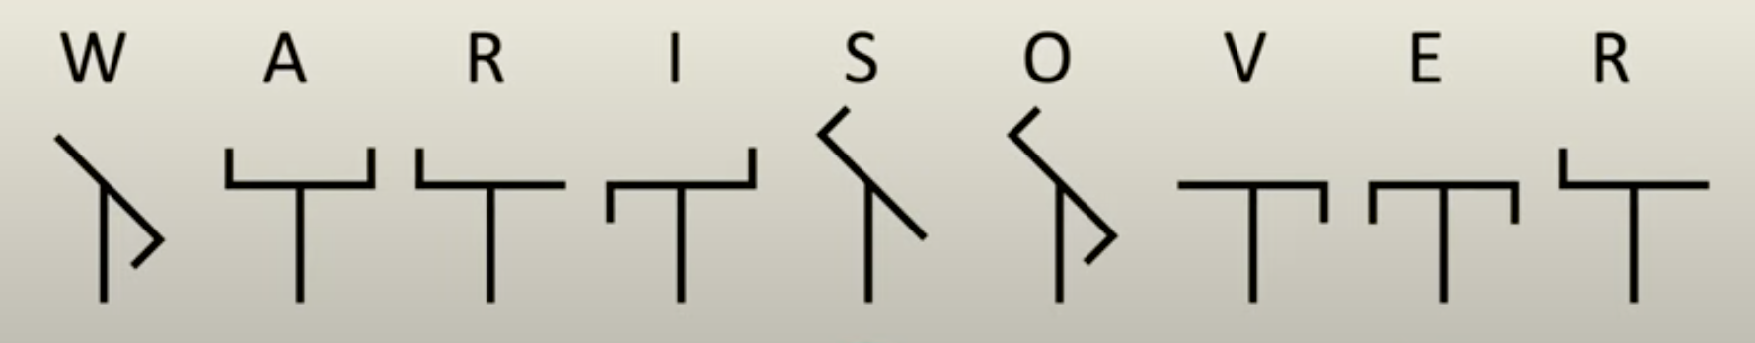
\includegraphics[width=0.5\textwidth]{lesson1/warisover.pdf}
    \label{fig: 1}
    \begin{center}
        \caption{例:腕木通信機}
    \end{center}
    
\end{figure}

例えば、このメッセージを伝えたい場合には、「War is over. (戦争が終わった)」こういうふうに示すんでしょう。こういう形にすることなんですが、どれぐらい大変なのでしょうかね。これは物理的に変更しなければならないんですが、配置によって変換することは
簡単かもしれないんですが結構人力が必要な場合もあります。
% Insert A -> R, W -> 10 
\begin{figure}[H]
    \centering
    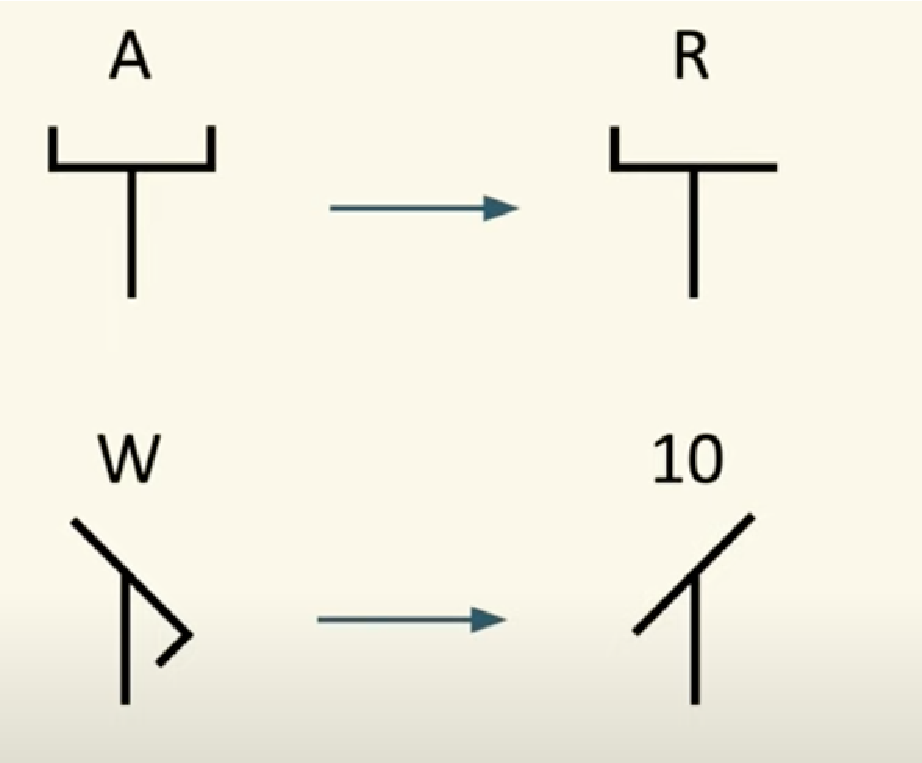
\includegraphics[width=0.8\textwidth]{lesson1/a_to_r.pdf}
    \label{fig: 1}
    \begin{center}
        \caption{例2:腕木通信機}
    \end{center}
\end{figure}
\textbf{Figure 1.16}ご示すのように、「A」から「R」なんですが、
は簡単な変換ですが「W」から「10」までの変換は結構難しい。この処理には、メッセージを伝えるためにはどのぐらいエネルギーを使うのか。どのくらい変換することが難しいのか。もちろん時間もかかるんです。
ナポレオンの手法は、記号が26個のアルファベットと10個の数字なんですが、
そのアルファベットと記号の組み合わせの数全部あわせると30億くらいあるんですけれども、そうすると、それが区別できるようにしなければならないので、それが結構複雑になるんですよね。
さて、モールス信号に戻ると、記号の数はどれぐらいになるでしょう。基本的に、 2つの記号しか使わないんですが、「ツー」と「トン」ですよね。英語では
ダッシュとドット。
% Insert U encoding
\begin{figure}[H]
    \centering
    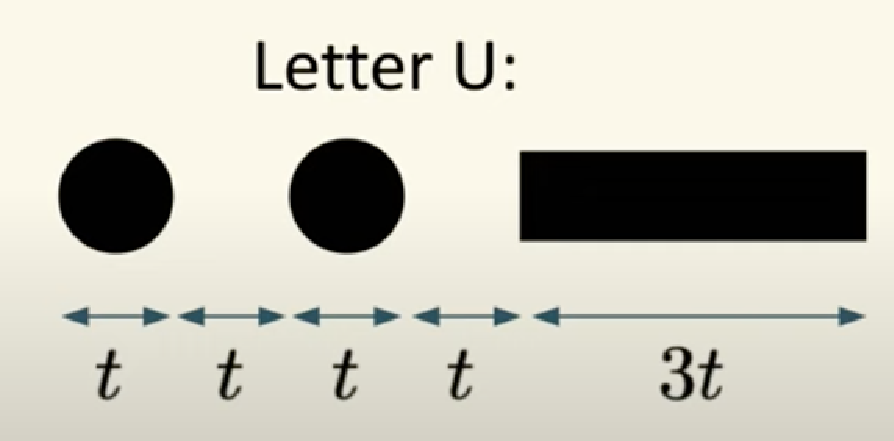
\includegraphics[width=0.8\textwidth]{lesson1/letter_u.pdf}
    \label{fig: 1}
    \begin{center}
        \caption{例:モールス信号}
    \end{center}
\end{figure}
\textbf{Figure 1.17}は\emph{U}のエンコーディングしたもので、「U」の記号としてはこれになるんです。
そうすると、短い時間はtを使って長い時間は3tを使うことにするんです。そうすると、早く変換できるようになるでしょう。
さて、こういう信号を伝えたい場合には、物理的にはどうしますかね?
\subsection{ビット (bit)}
% insert morse graph
\begin{figure}[H]
    \centering
    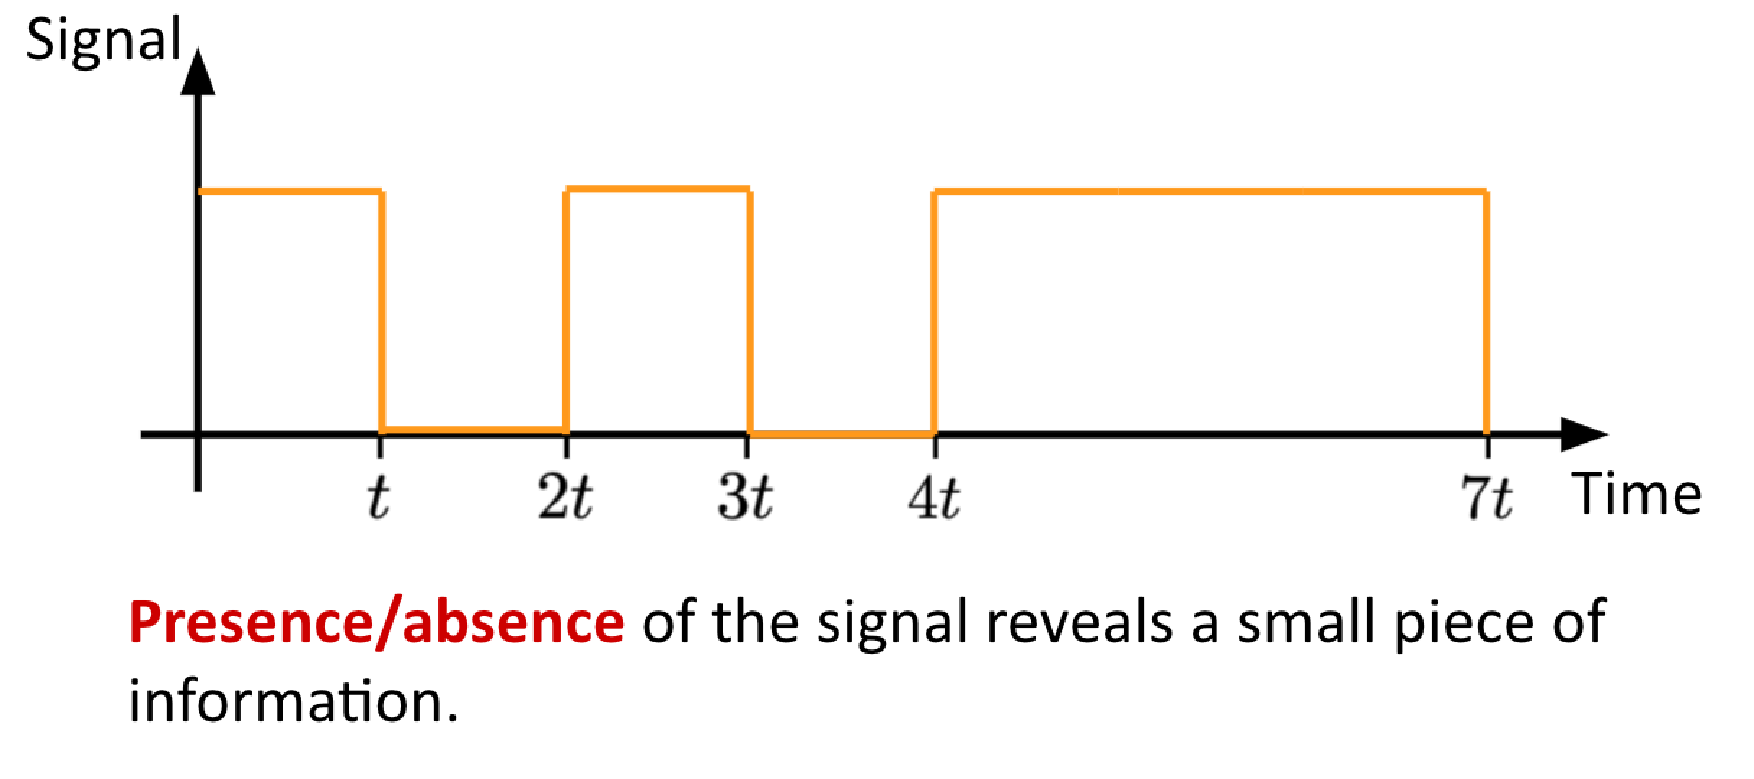
\includegraphics[width=0.8\textwidth]{lesson1/presence_abscence.pdf}
    \label{fig: 1}
    \begin{center}
        \caption{モールス信号のグラフ}
    \end{center}
\end{figure}
信号が\textbf{Figure 1.18}のふうにする場合があるんですが、例えばこれが左から右にいくと、これが時間軸なのですが、この信号は物理的には、例えば電圧なんです。
高い電圧が「1」、低い電圧が「0」の場合とすると0と1じゃなくて、この場合だったら「ドン」+「短いスペース」+「ドン」+「短いスペース」+「ツー」になるんですよね。この信号があるとない場合だけには、情報が伝われます。

一番ちっちゃい情報の単位は「ビット (bit)」になります。バイナリーデジット (binary digit)の略なので、これが「bit」となる。これが、コンピュテーションとコミュニケーション、計算と通信両方によく使う単位です。多分ご存知だと思います。これが「true/false(真偽)」と「yes/no」と「on/off」
のようないくつかのブーリアン(論理型)の型があるんですが、基本的にすべてを考えると、よく使う表現としては「0」と「1」なんですよね。
ビットの長所は「ノイズ(雑音)に強い所です。
\begin{figure}[H]
    \centering
    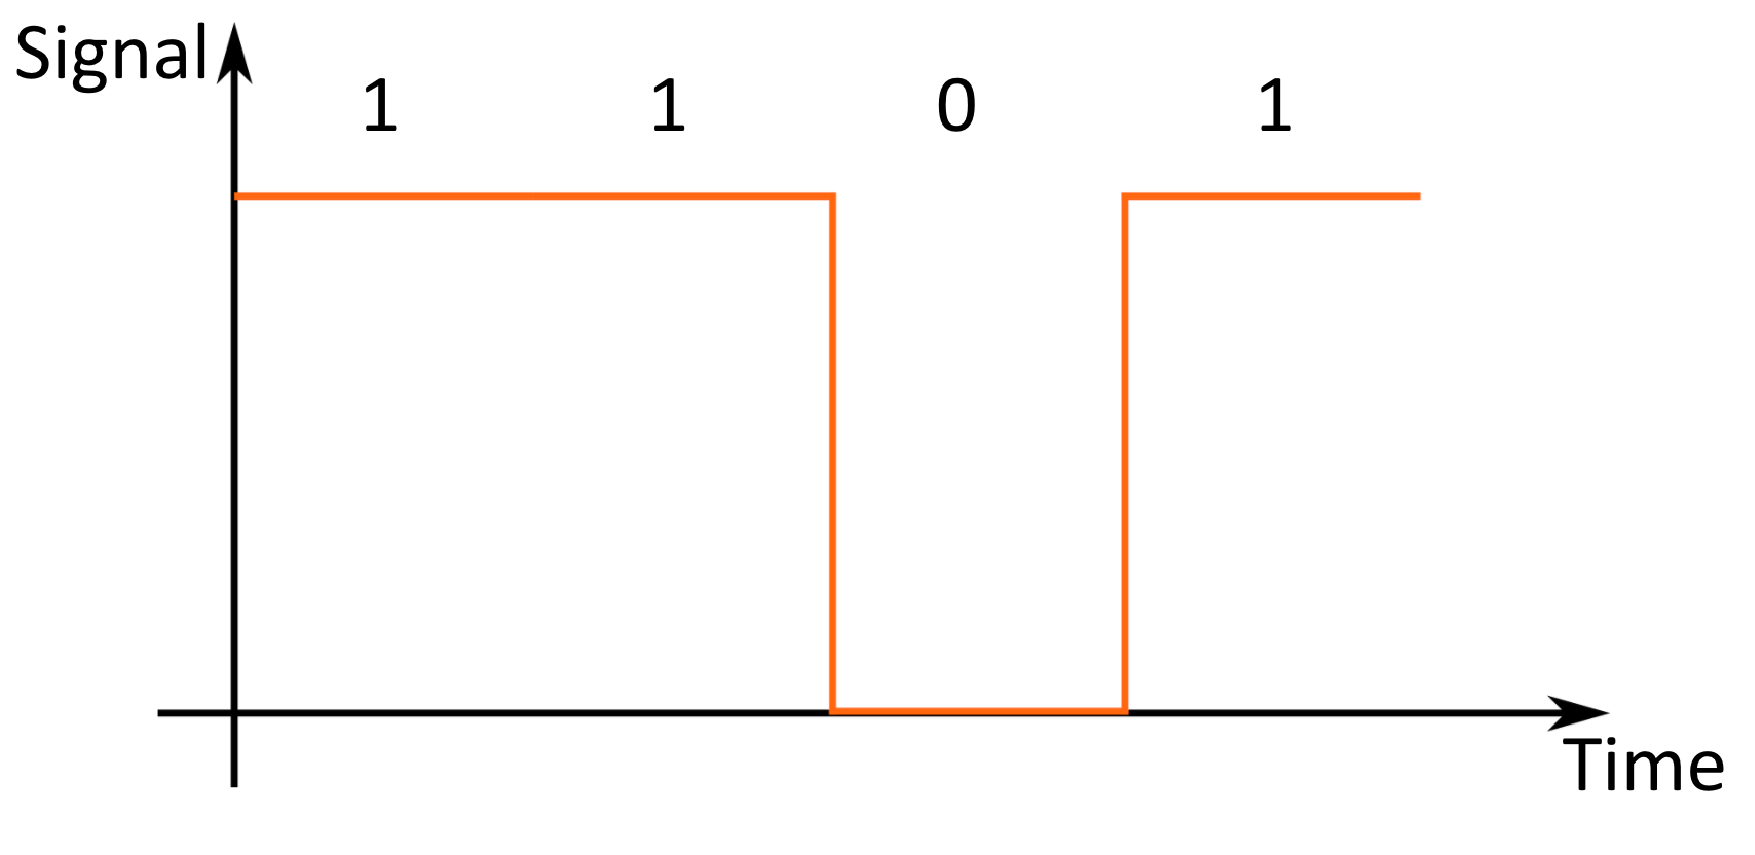
\includegraphics[width=0.8\textwidth]{lesson1/presence_abscence_bit.pdf}
    \label{fig: 1}
    \begin{center}
        \caption{ビットのグラフ}
    \end{center}
\end{figure}
この場合には、見える通りなんですが、この電圧が高いところと、電圧が低いところは結構離れてますよね?これが区別しやすいので、これが、今信号が高いところに「1」「1」で、低いところは「0」、高いところには「1」に戻る。
% insert graph w/ noise
\begin{figure}[H]
    \centering
    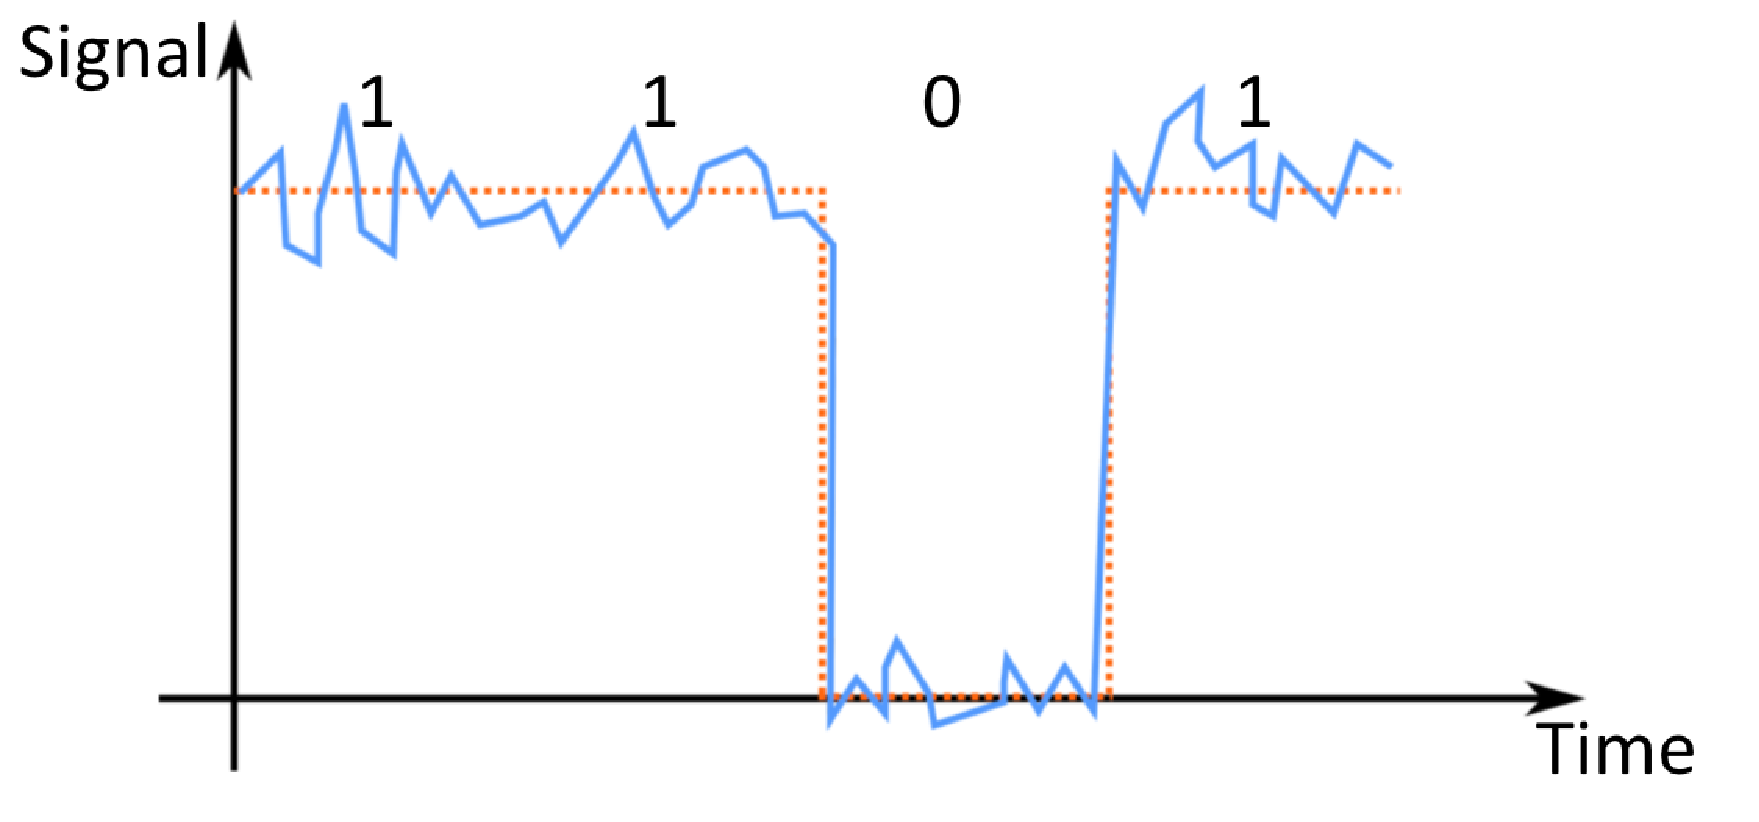
\includegraphics[width=0.8\textwidth]{lesson1/presence_abscence_noise.pdf}
    \label{fig: 1}
    \begin{center}
        \caption{ビットのグラフ}
    \end{center}
\end{figure}
ノイズがかかる場合を想定すると、\textbf{Figure 1.20}のふうになるかもしれないんです。それでも、上の段と下の段は区別はしやすいと考えられると思います。
\subsection{二進法}
さて、これがこういうふうに処理して、もともとあった信号の電圧に戻す場合はありますね。これが簡単にできるようでしょう?すると、さっきの最初の信号「1101」になってたんですがそれは取り出すことは簡単。

さて、このバイナリーノーテーション (binary notation) 。これを二進数の数え方でちょっと見てみましょう。たぶん見たことあると思いますが、念のために。
% insert bit permutations slide
\begin{figure}[H]
    \centering
    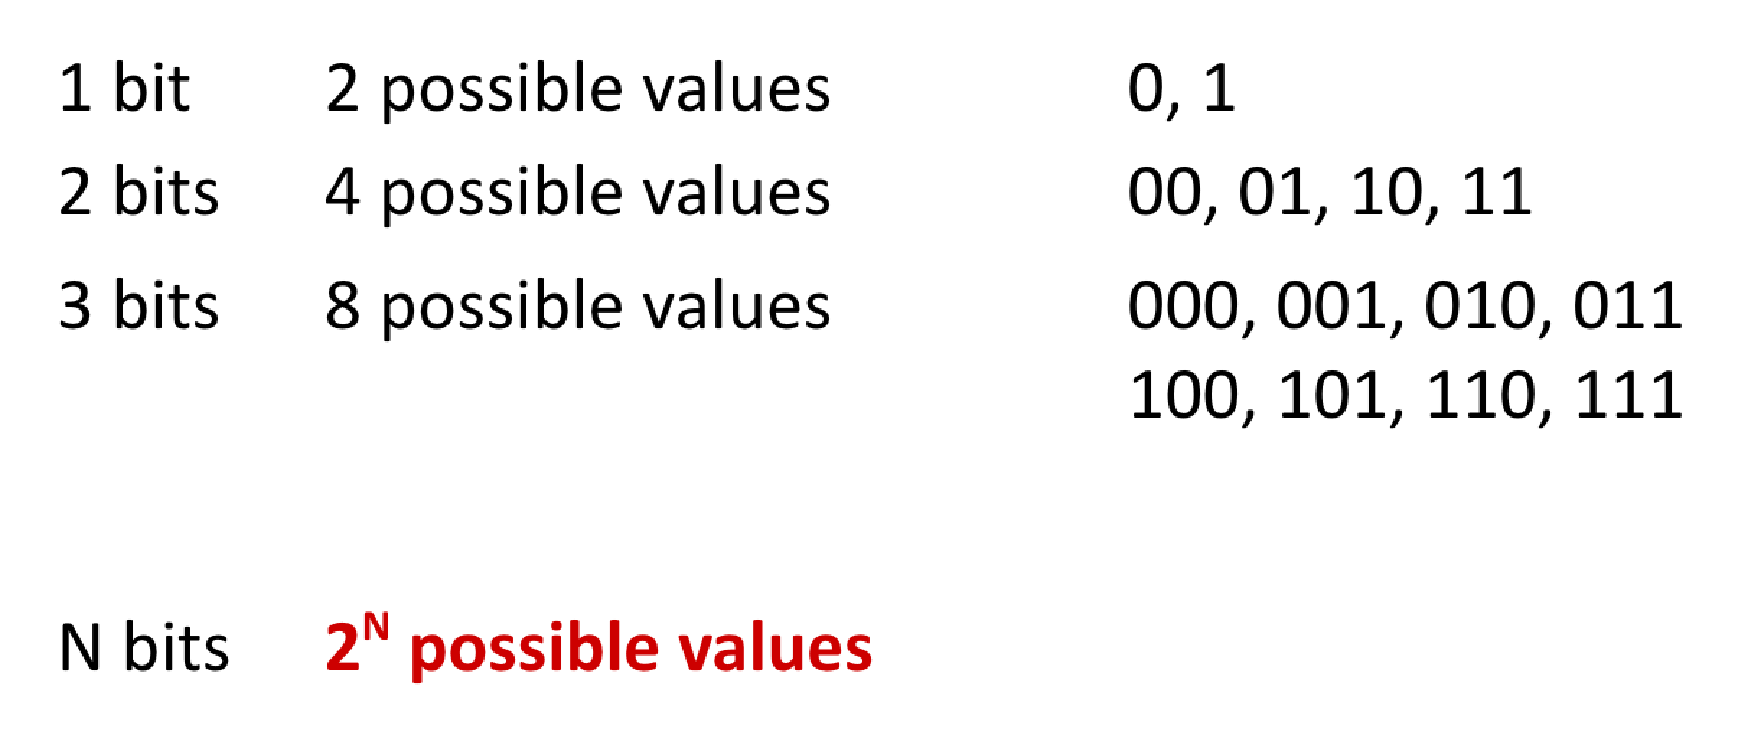
\includegraphics[width=0.8\textwidth]{lesson1/binary_notation.pdf}
    \label{fig: 1}
    \begin{center}
        \caption{ビットのグラフ}
    \end{center}
\end{figure}
一つのビットは2つの状態は可能でしょう。「0」と「1」
2つのビットだったら4つ。  「00」, 「01」, 「10」, 「11」。3つのビットだったら、8個の可能性がありますよね。000から111までで。まあ、これを繰り返すと分かると思います。けれども、
nビットを使うと2のn乗の状態は可能です。これが、2 のn乗のメッセージを伝えることは可能です。どうやって、これが十進。みなさんは小学生の頃から十進の書き方を学んでいるんですが、それがバイナリのことに変換できるんでしょう。
% insert decimal notation
\begin{figure}[H]
    \centering
    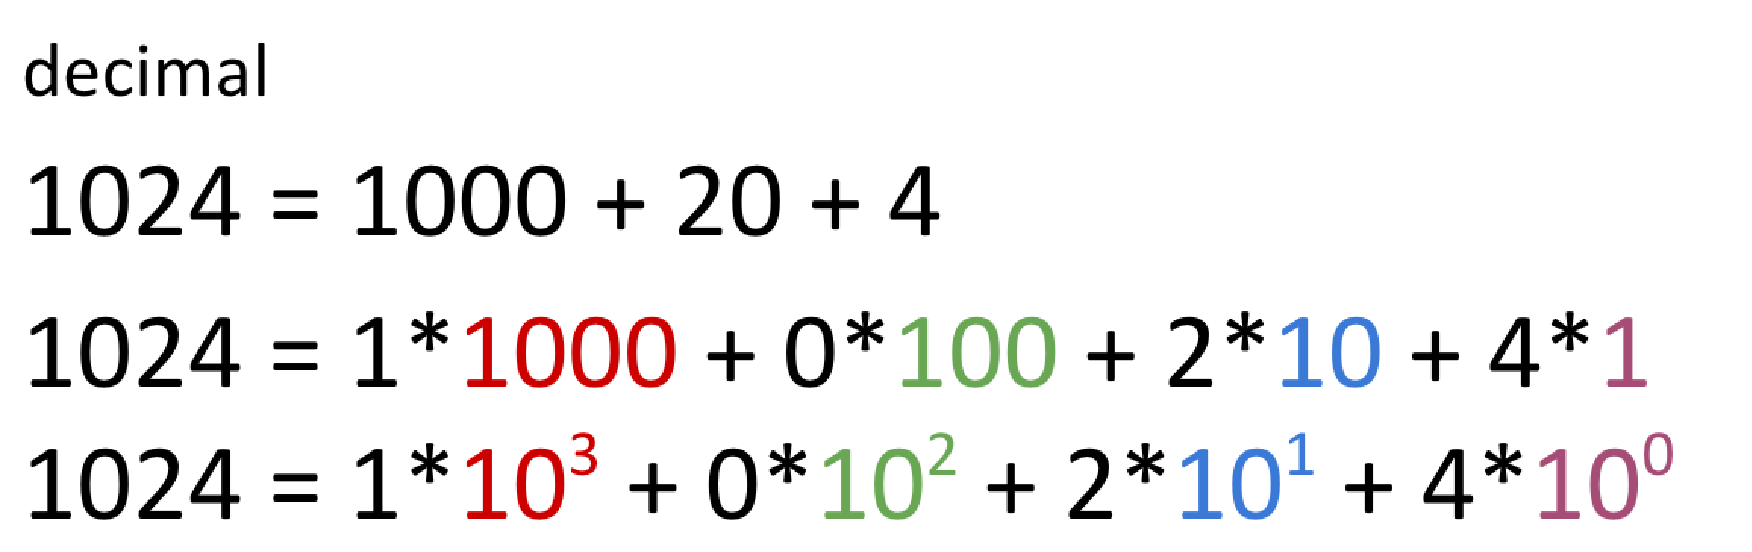
\includegraphics[width=0.8\textwidth]{lesson1/decimal_notation.pdf}
    \label{fig: 1}
    \begin{center}
        \caption{ビットのグラフ}
    \end{center}
\end{figure}
例えば、このデスマル(decimal、十進法)の場合には、
これが受信機なんですが、1024が「1000 + 20 +4」でしょう。そうすると、その最初の1が、「1 x 1000」という意味で、0が100の桁なのですが、その100の桁はないので、それは「0」を書いて続きで、2のところは、これが x 10なので、「2 x 10」最後には、「4 x 1」なんですね。もう一つの書き方にすると、「1 x 10の3乗」+「0 x 10の2乗」+ 「2 x 10の1乗」+ 「4 x 10の0乗」
これがバイナリー場合、二進でやると、これが「ベース 2 (二進数)」になるんですが、
「ベース 10 (十進数)」から「ベース 2 (二進数)」に変換することは可能です。

0:07:47.020,0:07:53.190
二進の例も見てみましょう。
% insert binary notation
\begin{figure}[H]
    \centering
    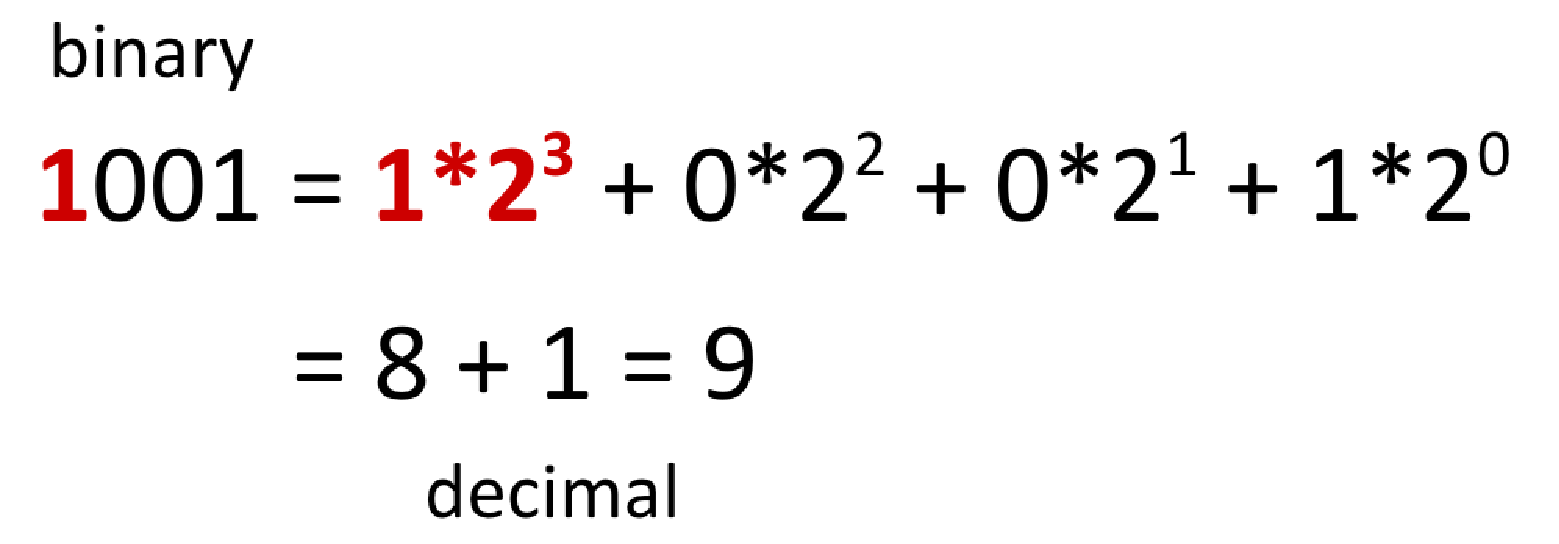
\includegraphics[width=0.8\textwidth]{lesson1/binary_ex.pdf}
    \label{fig: 1}
    \begin{center}
        \caption{ビットのグラフ}
    \end{center}
\end{figure}
これがバイナリーナンバーが「1001」だったら、それは「1 x 2の3乗」+「0 x 2の2乗」+ 「0 x 2の1乗」+ 「1 x 2の0乗」一緒なんですね。すると、その「1 x 2の3乗」が「8」なんで、一番下の桁は「1」になって、それで「8+1」は十進で 9となりますね。さて、ビットを使うことには、何が特徴で、何に役に立つのか?
\subsection{まとめ}
ビットの長所まとめ:
\begin{enumerate}
    \item 「ノイズ(雑音)に強い」
    \item 「エンコードする場合にもデコードする場合にも、結構やりやすい」
    \item 「処理することも結構簡単です」
\end{enumerate}
さて、こういう「ビット」が一番基本の概念でしょうかね?
まあ、「Yes!」なんですけれども。あとは「No!」なんですが。
「Yes!」は、古典(通信)の情報に結構使うんですが、Quantum(量子)の場合
「ビット」は一番基本の情報のUnit (単位)にはならない。そちらについては、今回のモジュールについては連続のステップでこれから説明します。



\section{量子通信}

情報が何かの物理のものに乗らなければでしょう。
それが電子でも光子でも電圧でも。さっきのナポレオンの腕木通信機では
形とか利用しているので、
それは物理的には何か利用しなければならないでしょう、情報を表示するためには。それが物理の手法で決まってるんです。
% Insert classical VS quantum slide
\begin{figure}[H]
    \centering
    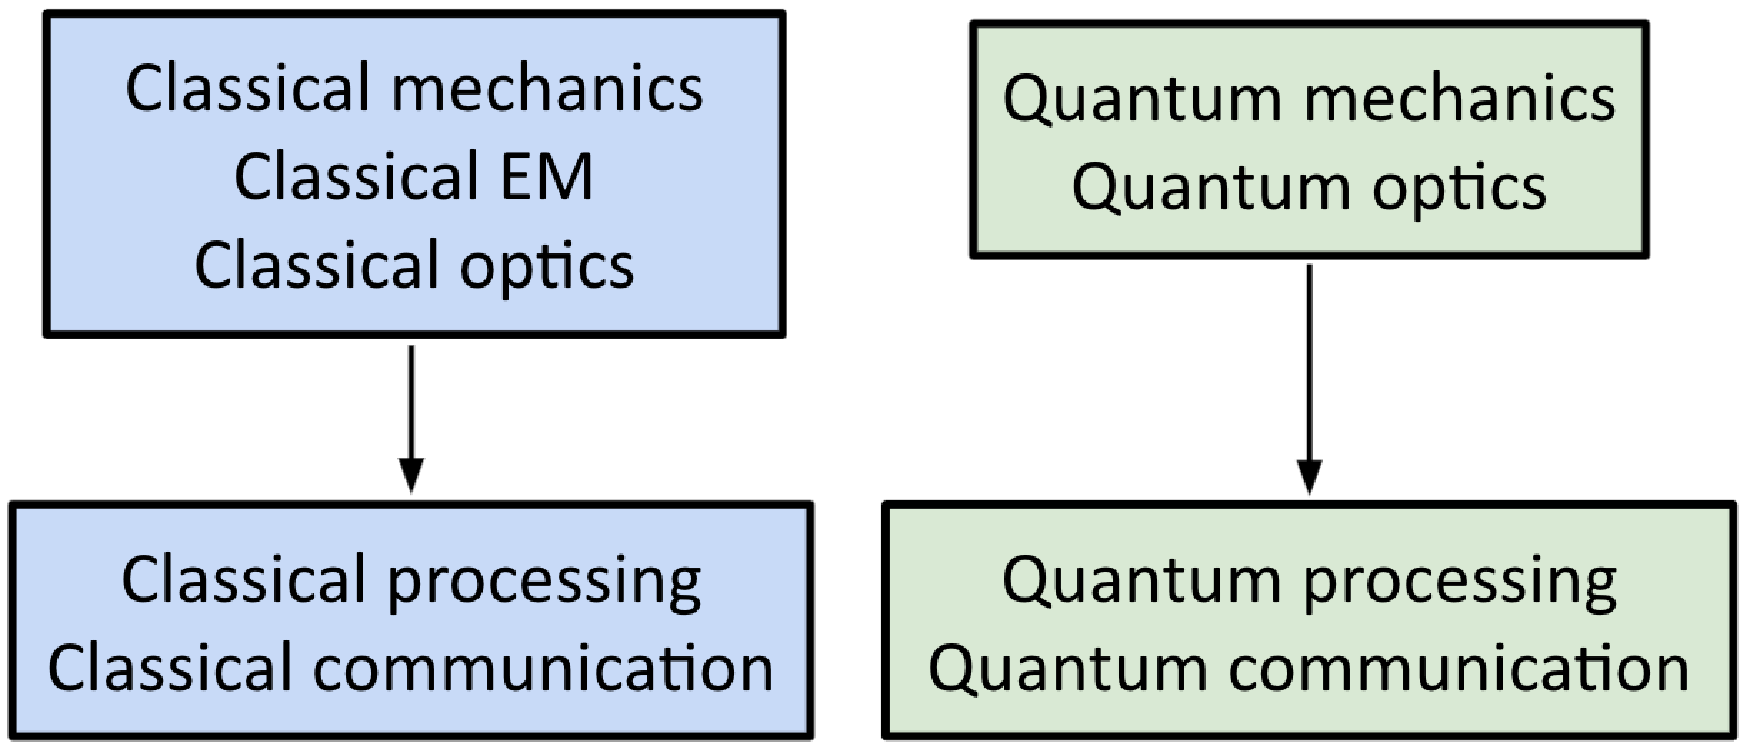
\includegraphics[width=0.8\textwidth]{lesson1/comparsion.pdf}
    \label{fig: 1}
    \begin{center}
        \caption{「古典」と「量子」}
    \end{center}
\end{figure}
決まってるんですよね、何ができるか、何が不可能か。物理的には制限されていますよね。そうすると、まぁ
古典(classical)のデータは、普通の古典力学と古典の光とか古典の光学とか、
古典のデータ処理とかによる古典通信に限られているんです。けれども、Quantum(量子)の場合だったら、量子力学 (Quantum Mechanics)と量子光学 (Quantum Optics)で決まっているんです。
そうすると、量子処理 (Quantum Processing)と量子通信(Quantum Communication)が行われます。

\subsection{古典力学の限界}
さて、量子力学が一番基礎の部分なんですよね。現在のこの宇宙でこれより精度が高い理論がないんですが。詳細なもので表現できるようになるでしょう。直感的ではないことに、結構行う場合があるんですが、まあそれがちょっと使えることが目的なんですね。これが実験ではすごく細かい精度まで調べてるんですが、それは精度はすごく高いんですよね。ですが、新しい手法と観測で見つかることになるかもしれないですが、それぞれの新しいデータの処理の手法が見つかる可能性はあると考えられると思います。実用的な理由で


なぜこれが使いたいのか、何が使えるのか?皆さんの使っている古典コンピュータと皆さんは携帯とかで見ているかもしれないし、ラップトップで見てるかもしれないんですがその中には一番基礎な、一番小さい信号を持つ措置とかとデータの処理する装置とかは、transistor(トランジスタ)と言いますね。そのトランジスタの数で、 一つの機能なんですがそれがコンピュータチップの
トランジスタの数が増えると、できる機能が増える可能性はあるんでしょう。
% Moore's law graph
\begin{figure}[H]
    \centering
    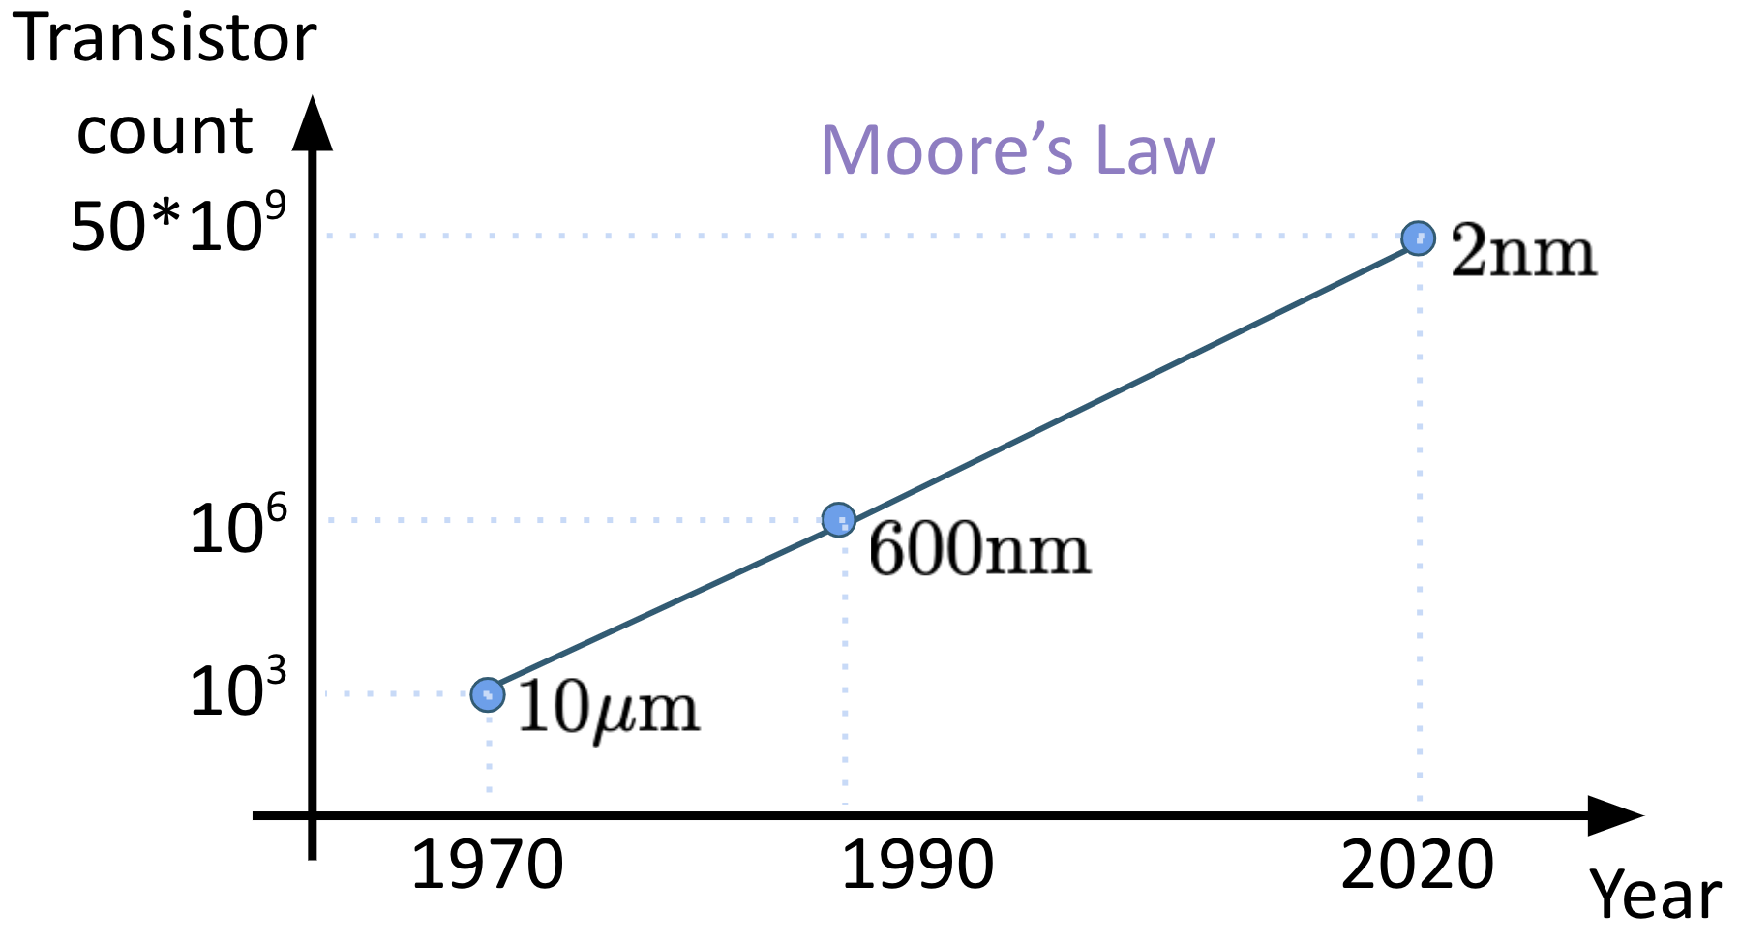
\includegraphics[width=0.8\textwidth]{lesson1/moore_law.pdf}
    \label{fig: 1}
    \begin{center}
        \caption{ムーアの法則}
    \end{center}
\end{figure}
1970年には最初のマイクロプロセッサーができたんですが、
それはインテルの4004のやつなんですが。2300トランジスタが入っていたんですね。すると1990年ぐらいには100個のトランジスタが、一つのチューブに入るようになってたし、2005年ぐらいには、10億トランジスタが入るようになりました。この進化が、\emph{「Moore's Law (ムーアの法則)」}と言いますね。
インテルのファウンダーのゴードン・ムーアさんが、1964年にそれについての論文を提出したんですけれども、「各時期には一つのチップに入るトランジスタの数が倍になるでしょう。」と書いていました。最初の提案は、2年間か3年間なんですが、一番速く進化してた時代には、それが18ヶ月くらいには倍になってたんですね。でもそれが最近は段々その進化が遅れるようになっているんですが。一つの理由としては、そのトランジスタの大きさが変わっているんでしょうね、その技術の進化として。
技術の進化はチップの大きさがあまり変わらないんですね。
時代から時代に進むと。例えば、一つのチップは大体親指の爪ぐらいの面積なんですよね。2cm x 2cmぐらいなんですが、それがさっきの進化の説明した通りで、入るトランジスタの数が増えることなんですが、トランジスタの大きさが段々小さくなるんですよね。その1970年代のトランジスタが、10マイクロメートル(μm)ぐらい。一つのマイクロメートルは1m の100万分の1なんですが。
進化すると、今の時代には、数ナノメートル(nm)。一つのナノメートルが
マイクロメートルの1000分の1ですね。メートル(m)の1000分の1が、ミリメートル(mm) で、ミリメートルの1000分の1がマイクロメートルになって、マイクロメートルの1000分の1がナノメートルになるんですね。

それが続くと、もう一番小さいトランジスタの部分が数ミリしかないんですが、その数ミリの大きさで、\textbf{トランジスタがほぼシリコンの原子の大きさ}ぐらいになっているんですね。シリコンの水晶の中には、原子と原子の距離が0.5ナノメートルぐらいしかなってないなら、2ナノメートルになるなら、それが4個になります。その進化はそろそろ終わってしまうんですよね。それが原子の一個下のトランジスタを作る手法がわからないので。
\subsection{唯一の救世主:量子力学}
すると、量子力学によってどのような新しい展開が生まれるでしょうか?
新しい概念、新しくできることはどのくらい変わるでしょう?
\textbf{重ね合わせ (superposition)}を使うんですが、それが波を使って、その波の特徴を使って重ね合わせの状態のようになることなんです。それは次のレッスンで説明します。True and False (真偽)、On and Off (オンとオフ)
Yes and No(イエスとノー)をそれが表示できるようになるんです。

次の概念が\textbf{エンタングルメント (entanglement)}なんですが、そのエンタングルメントは\textbf{「量子もつれ」}と言いますが、それは古典の場合にはないんで、それが重ね合わせを使って、複数の量子とビットとか使って、離れている距離で重ね合わせを作ると、
それがエンタングルメントになる場合があるんですが、この次のステップで説明します。これが\textbf{Correlation(相関関係)}になるんですけれども、
その相関関係が古典より強くなります。そうすると、新しい通信の手法が生まれます。そうすると、これが量子ネットワークの基底になるんです。それが使えるようになる量子通信を目指しています。
\subsection{まとめ}
さて、この量子通信は難しいんでしょうかね?まあ、すごく壊れやすい状態なんですけれども、それが\textbf{「decoherence(デコーヒレンス)」}と言います。デコーヒレンスは古典のノイズと同じ概念なんですが、それがさっきの話をしてた重ね合わせと量子もつれが破壊される場合があります。そうすると、新しいプロトコルを開発しなければなりません。それが、このモジュールの一つの目的としては、それがどうやって開発されているのかを説明することです。

これが\emph{challenge(挑戦)}かもしれないんですけれども、これが\emph{oppotunity(機会)}にもなりますよね。これが良い機会になるので、量子の特徴を使って新しいシステムを作る事は可能です。これが\emph{interdisciplinary(学際的な、分野を横断した)}ことなんですけれども物理学者も必要だし、数学も必要だし、Electronic Engineers(電気・電子技術者)も必要だし、Computer Scientists(計算機学者)も必要だし、Computer Engineers(計算機技術者)も必要なんですね。



\section{量子時代のセキュリティ}
\subsection{紹介}
量子技術がいろいろな分野に影響するんです。
例えば、
\begin{enumerate}
    \item 材料の科学
    \item 測定の手法
    \item 医療系
    \item 人工知能
    \item
\end{enumerate}
このステップは量子通信についてのテーマですから、セキュリティの方を説明したいと思います。

\subsection{古典通信VS量子通信}
% insert unencrytped msg pic (milk please)
\begin{figure}[H]
    \centering
    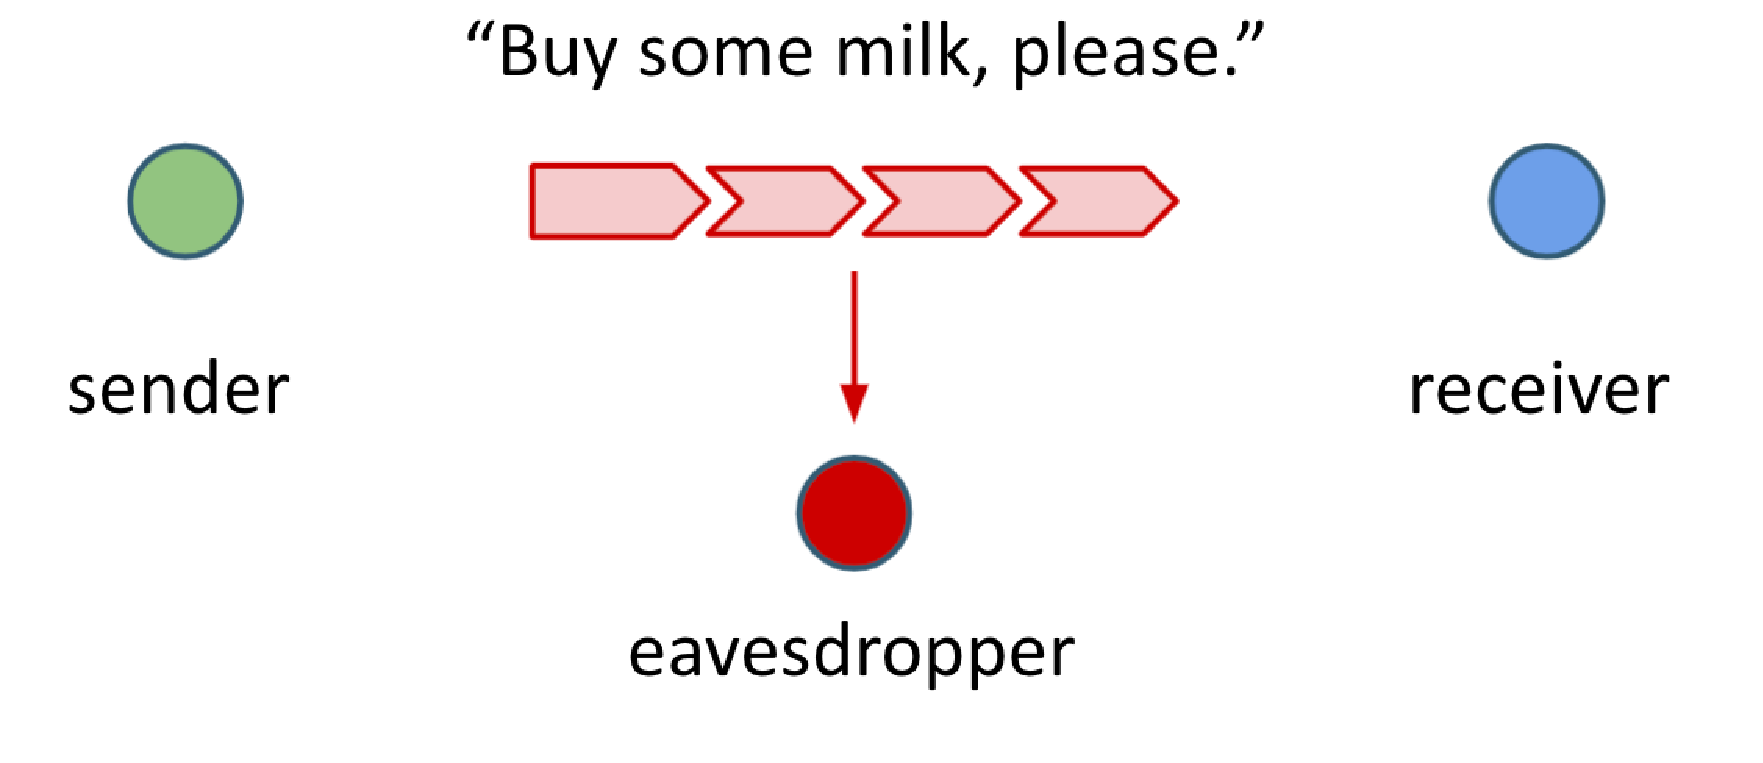
\includegraphics[width=0.8\textwidth]{lesson1/milkplease.pdf}
    \label{fig: 1}
    \begin{center}
        \caption{暗号無しの通信:つまらない内容}
    \end{center}
\end{figure}
まずはメッセージを送りたい状況なんですが、それが暗号されてない場合だったら送信者と受信者がいるんですが、
こういう赤いところは、これは\textbf{チャンネル(通信路)}なんですが、
そのチャンネルにメッセージを通して、盗聴者がいたら、その盗聴者がメッセージをコピーして内容が完全に読めることはできるでしょう。あとは、内容の変更も可能なんですが、この場合のプライバシーについて議論したいと思います。
例えば、メッセージの内容が「牛乳を買ってきてください」とかいうと、
その内容はもしかして誰かがその内容をわかって入れば問題ないかもしれないんですが、他の例にすると、例えば
% insert credit card info 
\begin{figure}[H]
    \centering
    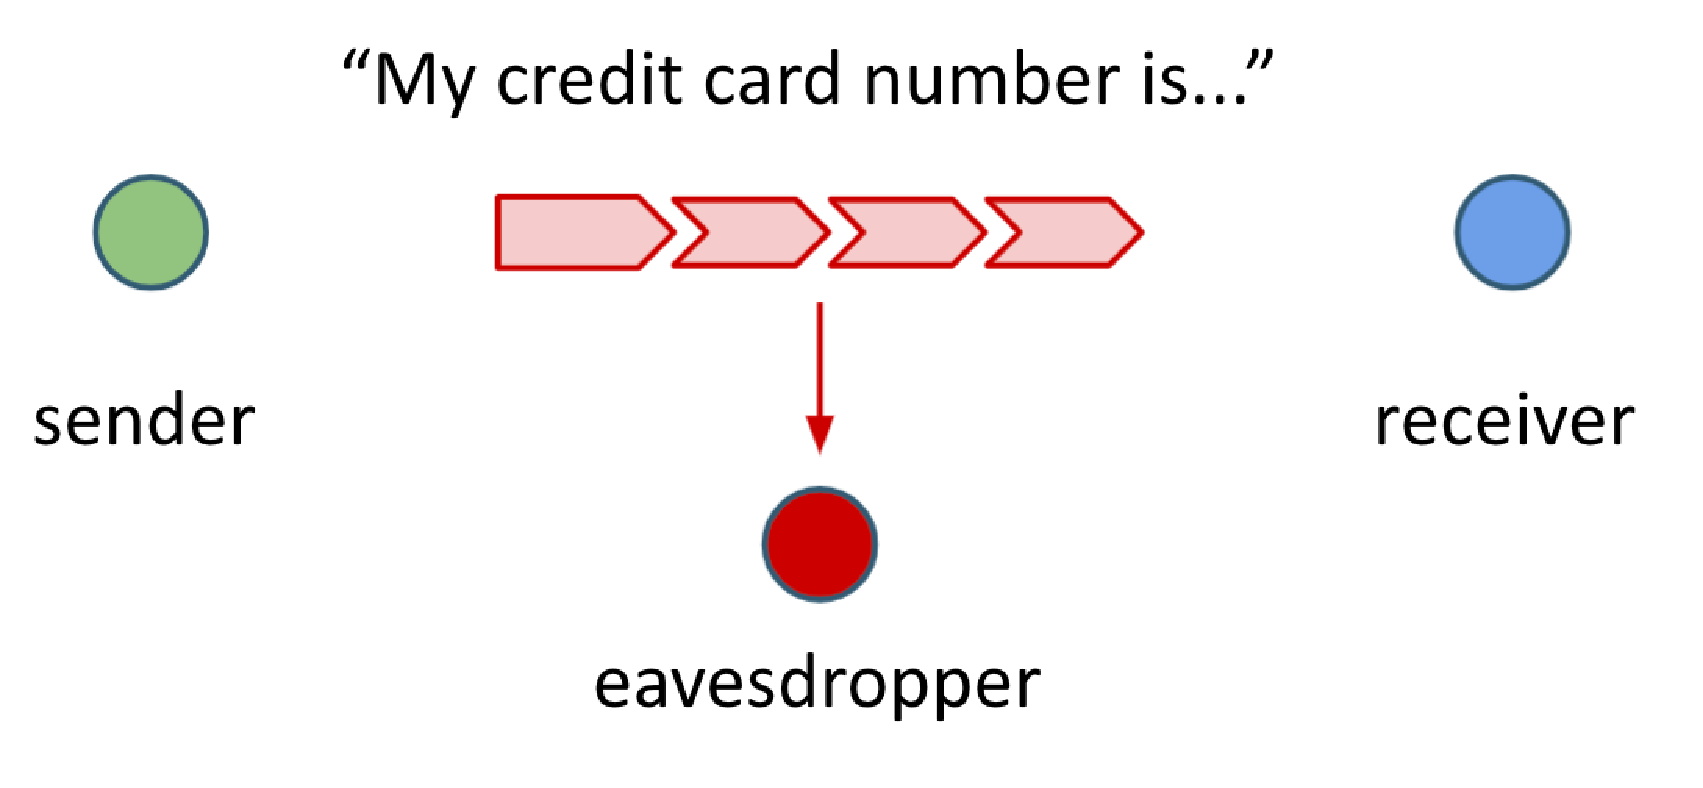
\includegraphics[width=0.8\textwidth]{lesson1/creditcardinfo.pdf}
    \label{fig: 1}
    \begin{center}
        \caption{暗号無しの通信:大事な内容}
    \end{center}
\end{figure}
「僕のクレジットカード番号はこれです」とメッセージを送ってたら、
盗聴者はそれが盗聴したら、そのクレジットカードを使えるようになるかもしれないので、困る場合はありますよね。

さて、これが大きな問題になるかもしれない。
なので暗号が開発されたんですが、その暗号は何千年間の歴史があるんですが、すごく軽く説明をしましょう。
% encrypted msg pic.
\begin{figure}[H]
    \centering
    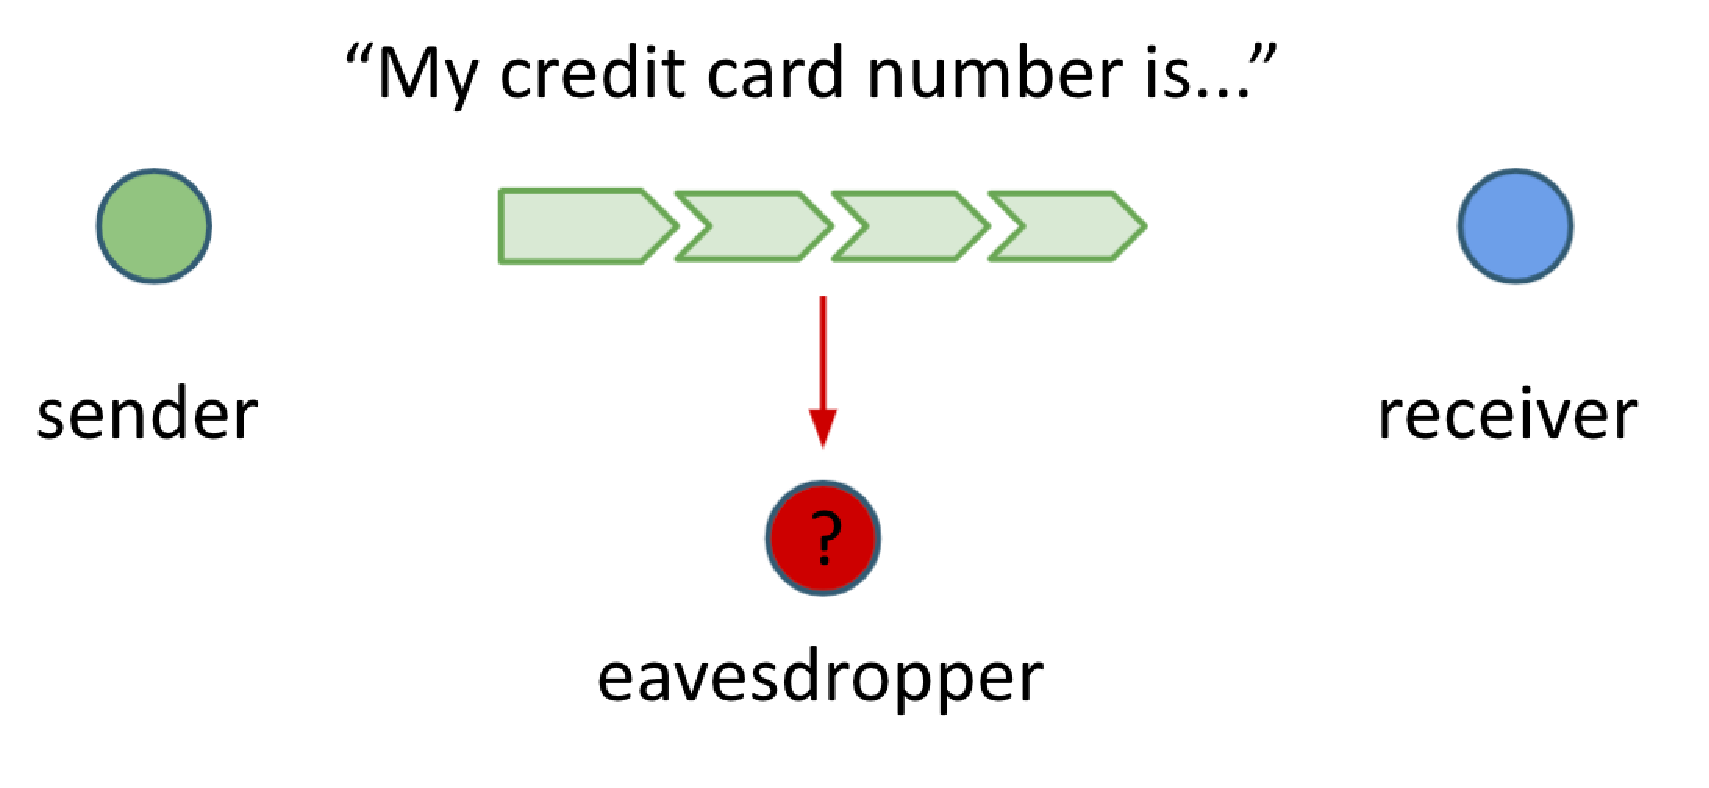
\includegraphics[width=0.8\textwidth]{lesson1/credit_card_info_eavesdropper.pdf}
    \label{fig: 1}
    \begin{center}
        \caption{暗号化された通信}
    \end{center}
\end{figure}
例えば、これだったら送信者から受信者までメッセージ送りたいんですが、その送っているメッセージが暗号化されている場合なら内容は盗聴者は読めないので、安全と言えるでしょう。しかし、それが完全に安全と言えないんですよね。暗号の問題は解読することは不可能ではないんですが、
数学的には問題には関連する指数があるんですが、それ(暗号の問題を)を解決することは難しいんですが、不可能ではない。
解読の手法によるんですが、基本的にはここまで考えてみましょう。
% insecure channel pic.
\begin{figure}[H]
    \centering
    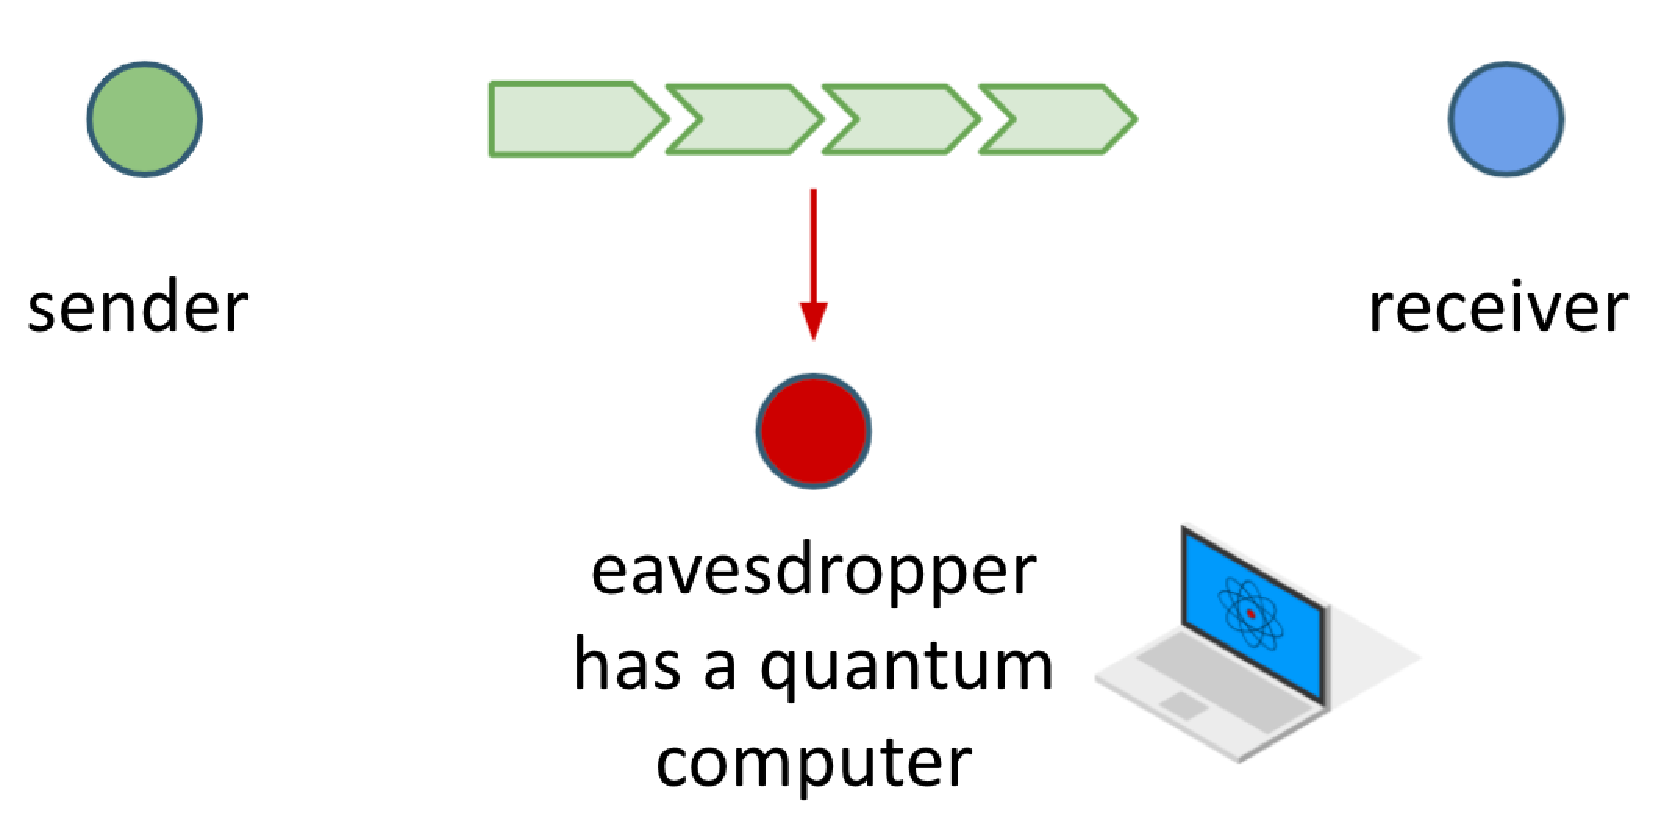
\includegraphics[width=0.8\textwidth]{lesson1/eavesdropper_Q_comp.pdf}
    \label{fig: 1}
    \begin{center}
        \caption{量子コンピューター持つ盗聴者}
    \end{center}
\end{figure}
例えば、その盗聴者が量子コンピュータを使えるなら、数学的な暗号手法を解決する可能性はあるんですが、そうすると例えば、これから勉強することなんですが 、
ディフィー・ヘルマンの鍵交換とかのシステムについては、量子コンピュータが解決する可能性があります。そうすると、このチャンネルがセキュアなチャンネルじゃなくて、インセキュア(安全でない)チャンネルと呼びましょう
量子チャンネルを使っていたら、 量子コンピュータじゃなくて、

このチャンネルを量子チャンネルに変更したらある手法を量子暗号、量子鍵交換の技術を使ってたら解読は不可能にはなるんですが、盗聴者がいるかどうかは重要なメッセージを送る前に発見することは可能です。
% Quantum Channel "STOP" pic
\begin{figure}[H]
    \centering
    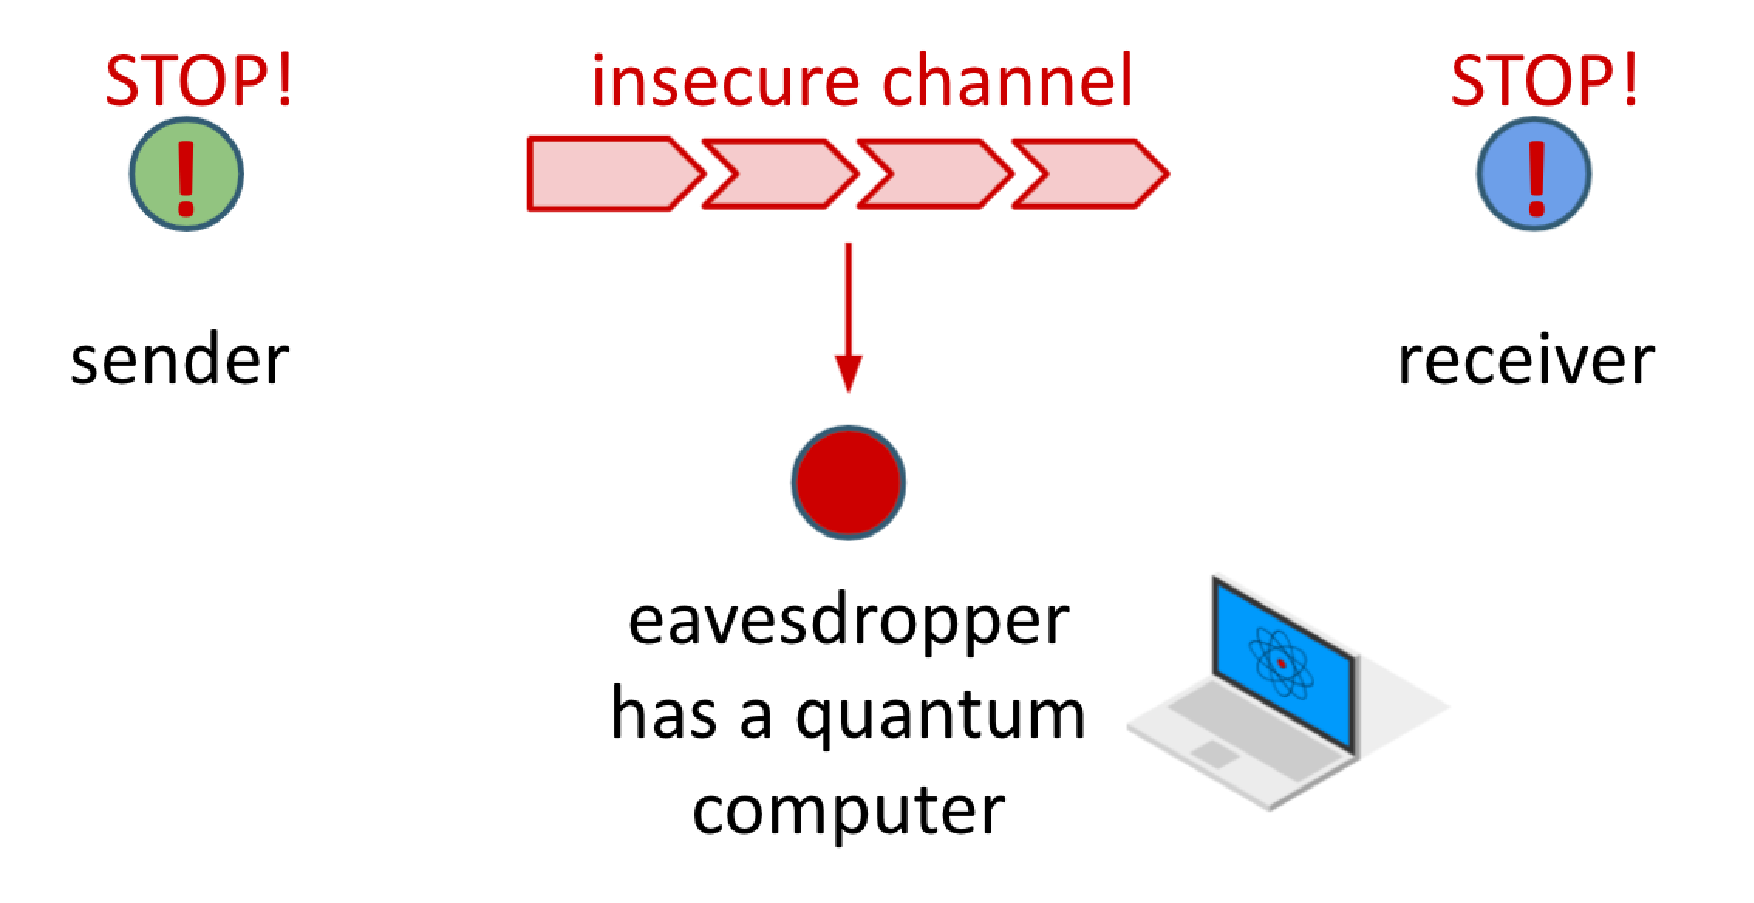
\includegraphics[width=0.8\textwidth]{lesson1/insecure_channel_stop.pdf}
    \label{fig: 1}
    \begin{center}
        \caption{量子チャンネル:通信中止}
    \end{center}
\end{figure}
送信者と受信者は盗聴者がいることがわかるようになります。盗聴者の存在に気付く送信者と受信者はその通信を止めることができます。


\section{モジュールの概要}


今学期には何を勉強するでしょう。
% insert course overview pic
\begin{figure}[H]
    \centering
    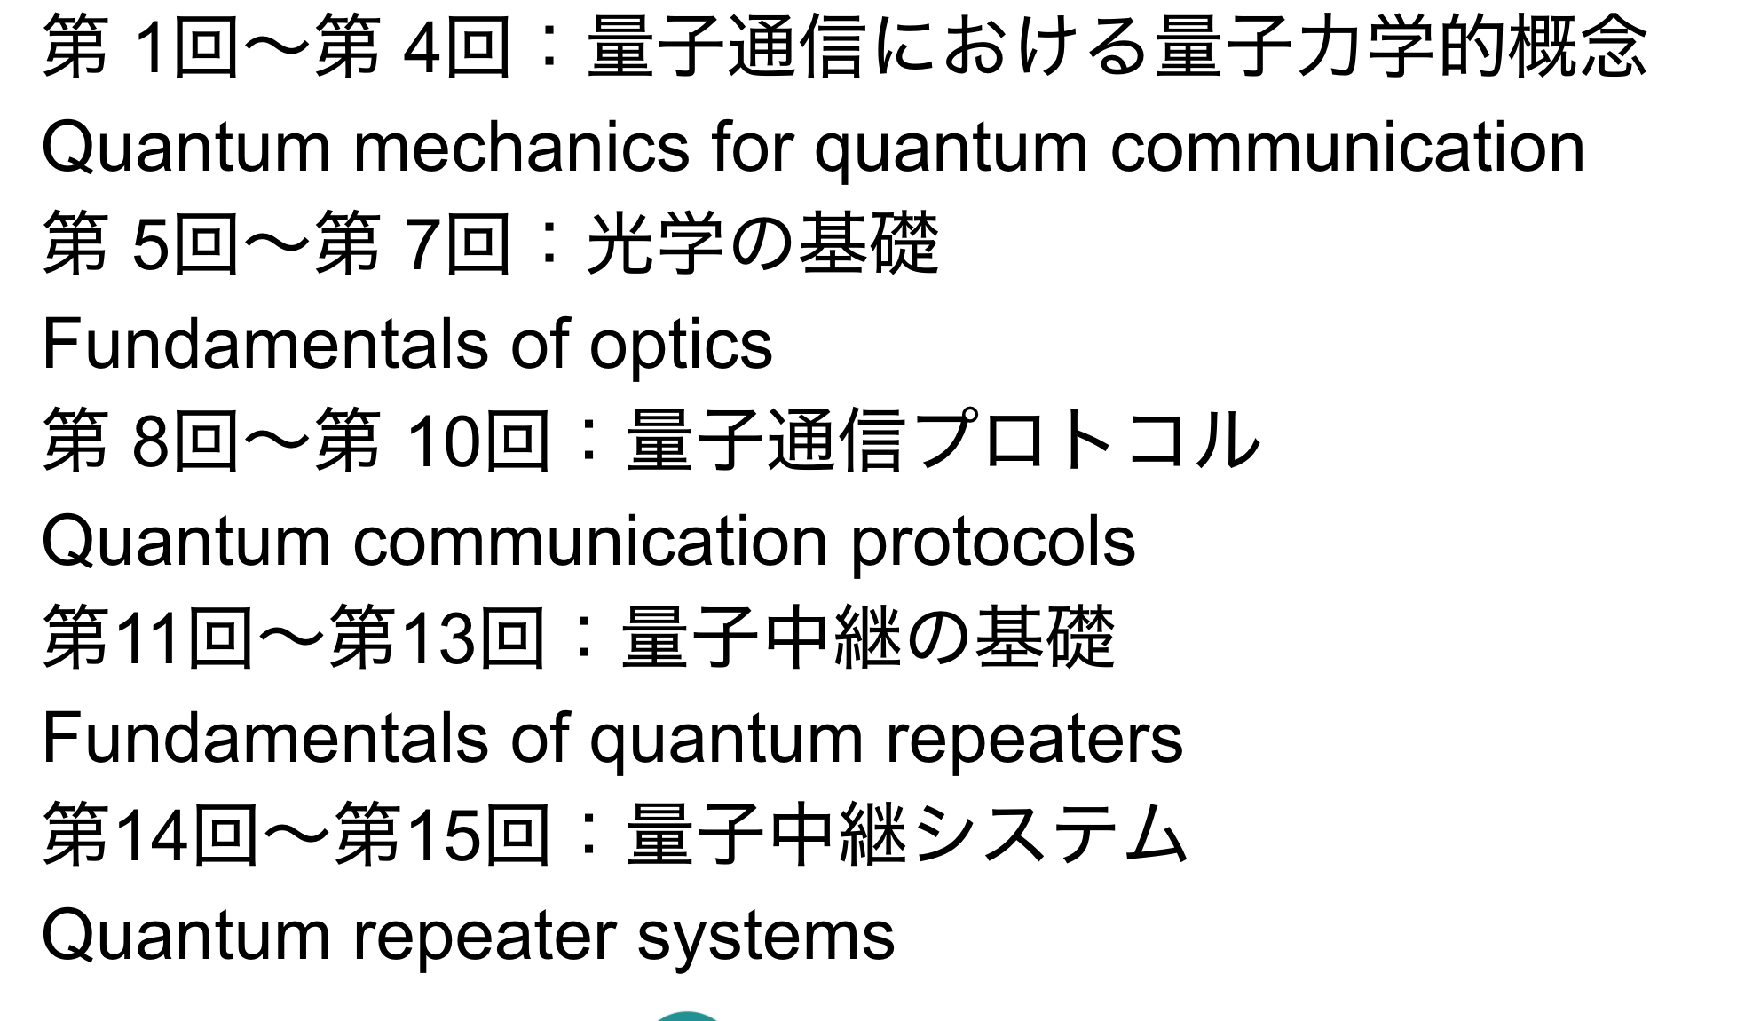
\includegraphics[width=0.8\textwidth]{lesson1/module_overview.pdf}
    \label{fig: 1}
    \begin{center}
        \caption{モジュールの概要}
    \end{center}
\end{figure}
このモジュールにはいくつかのテーマが
あるんですけれども、1、2、3、4、5のテーマに分けているんです。
レッスン1から4までは量子力学なんですが、深くは勉強しないんですが軽く紹介することとしています。レッスン5から7までは、光学の基礎なんですが、レッスン8から10は、量子通信の基礎。それは量子鍵配送等を含むことです。レッスン11から13は、量子リピーター、量子中継器の基礎なんですが、14と15はその量子中継器のシステムについて議論します。
\subsection{前提について}
% insert pre-requisities slide 
\begin{figure}[H]
    \centering
    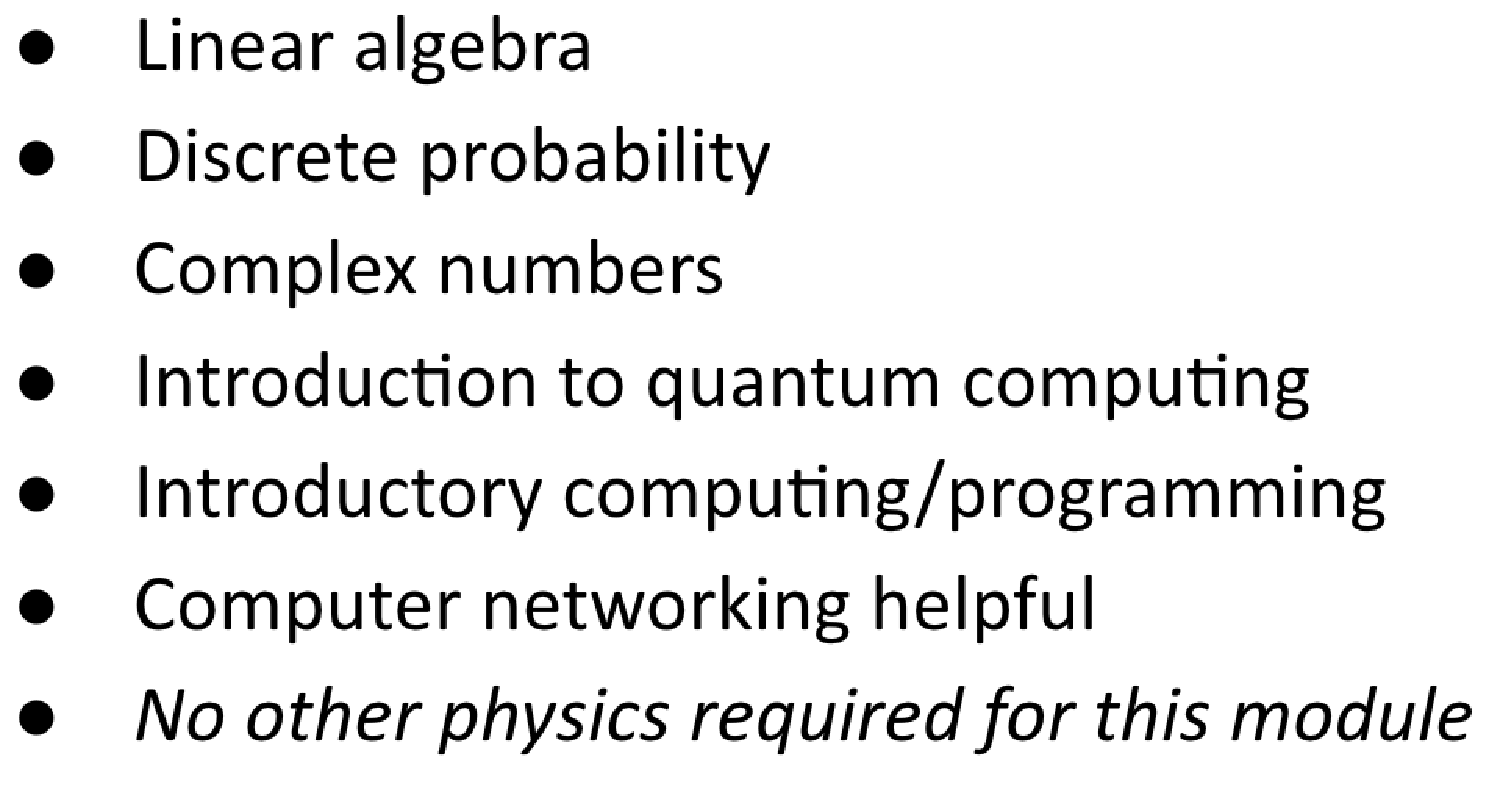
\includegraphics[width=0.8\textwidth]{lesson1/prereqs.pdf}
    \label{fig: 1}
    \begin{center}
        \caption{コースの前提}
    \end{center}
\end{figure}
これは何を前提としているのでしょう?前提か、一緒に勉強しているのか、
進みながらもできることにはできると思うんですがまずは\emph{線形代数}。それがすごく重要なんです。あとは、\emph{確率}。これが簡単な方だけなんですが。あとは、\emph{複素数}。それも、\emph{オイラーの方程式}も重要なんです。あとは、並列で\emph{量子計算の基礎}を勉強した方がいいと思います。これがコンピューティングシステムズの内容なので、
基本的にプログラミングができることも重要だと思います。\emph{Pythonの言語}は、ちょっとだけは使うことにはするんです。
そして普通の\emph{古典コンピューターネットワーク}も重要なんです。
インターネットとかTCP/IPとかネットワークの基礎のことを勉強するということは重要。それから、物理学はあんまり内容は深くはしませんが、
重要な量子力学は最初の方には説明するのですが、
それ以外は、特別な物理学の授業を履修しなくても結構です。

さて、その量子計算機の入門としては、いくつかのオプションがあるんですけれど一つは、慶應大学の開発した「Understanding Quantum Computers
(量子コンピュータの理解)」のMOOC。オンラインコースで、これが高校生レベルから学部の1年生あたりのレベルなんですが、数学はあまり使ってなくて、最初のものは英語なんですが、日本語、タイ語、インドネシア語の字幕と記事もそれらの言語に翻訳されているものがありますから、安心して使ってください。

% Rod videos pic
\begin{figure}[H]
    \centering
    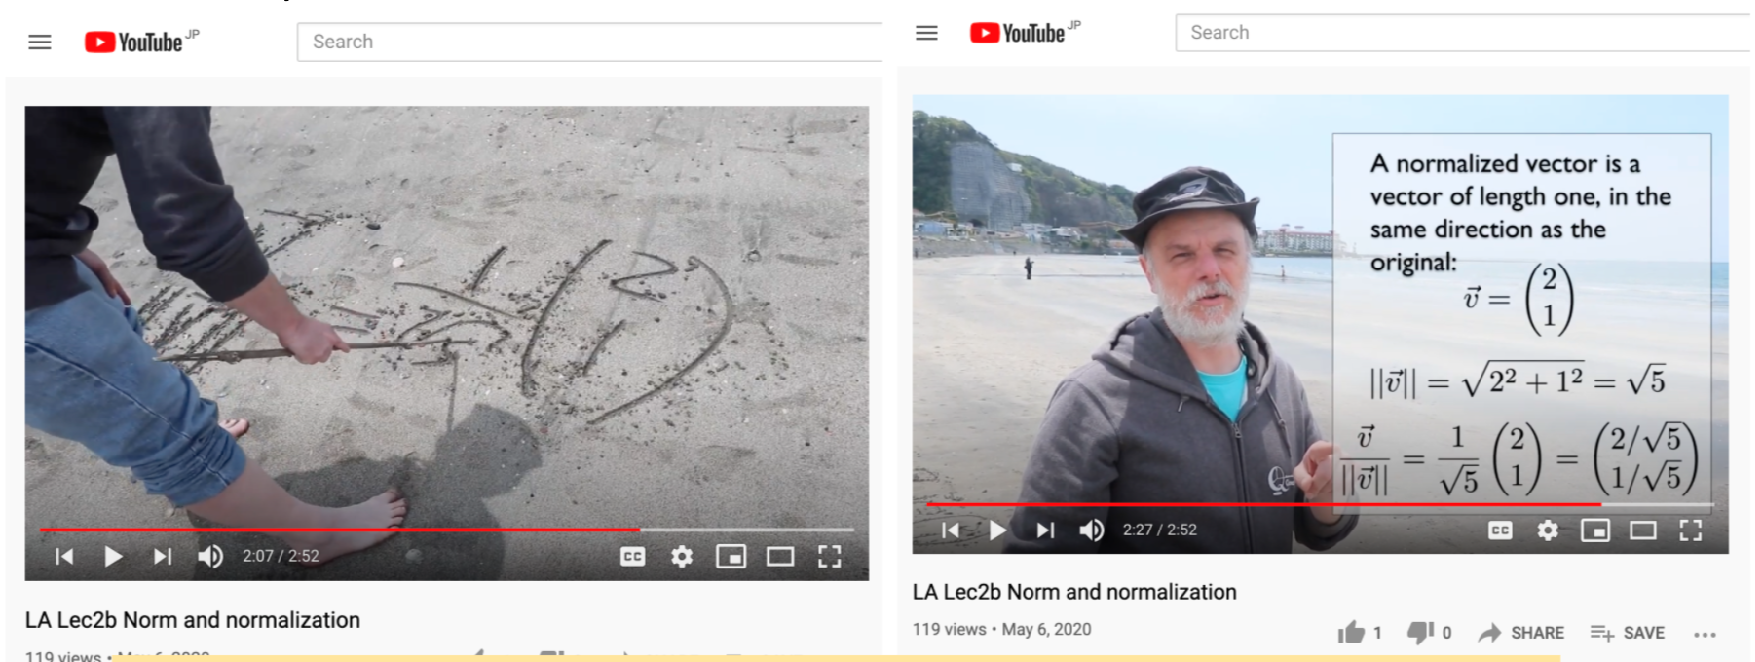
\includegraphics[width=1.1\textwidth]{lesson1/lin_alg_vids.pdf}
    \label{fig: 1}
    \begin{center}
        \caption{先生の線形代数ビデオ}
    \end{center}
\end{figure}

さて、線形代数としては、それもいろんなところで学べるのですが、
他の選択肢がないなら、慶應大学の湘南藤沢キャンパスで線形代数の授業は
そのビデオが、Youtube にアップされてますので、こちらのURLでアクセスしてください:
\url{http://www.youtube.com/playlist?list=PLibMrvP9xUbeWZ1pCKnbTn2FO-c1PqHZr}.

大体はこの内容なんですが、もちろんそれをやりながら見えてくるんですけれども、これから量子通信の基礎を楽しくワクワク勉強しましょう!
